\documentclass{article}
\usepackage{graphicx}
\usepackage{placeins}
\usepackage{hyperref}


\title{Mini-Project 3: SeeDB}
\author{Anushree Mehta, Benjamin Mende, Ramya Tammisetti }
\date{May 5, 2018}

\begin{document}

\maketitle

\section*{Description}
For this project, we implemented several algorithms outlined in \textit{SeeDB: Efficient Data-Driven Visualization Recommendations to Support Visual Analytics}. SeeDB is a visualization recommendation engine that operates on single-table databases to propose potentially interesting visualizations of the data to help with exploration. The innovation of this paper is proposing several optimizations to explore all necessary data for an interactive application, as well as proposing a measure of interestingness. 
 
We tested our simplified reproduction of SeeDB with the US Census Income Dataset, which is divided into a training and test set. Because this split is not relevant to SeeDB, we have opted to combine these into a single dataset. While the authors of SeeDB did conduct experiments using this dataset, we do not expect to find the same results because they reported this data as having only 21,000 rows while we have a version with 48,000.

\section{Tools}
We used a combination of PostgreSQL and Python in our implementation, executed using Psycopg2, a DB API 2.0 compliant PostgreSQL driver that is actively developed. Scipy and Matplotlib were used to compute utility measures and for visualization respectively. Additionally, all our code and implementation is hosted on github at \url{https://github.com/abmehta/SeeDB\_645Project}

\section{Methods}
\subsection{Target and Reference Data}
SeeDB works by comparing the distribution of queries run on a target dataset to the same query run on a reference dataset. We partitioned the US Census Income dataset into target and reference data based on the marital status of US adults with the target being all rows representing married individuals and the reference being all rows representing unmarried individuals. Specifically, we selected as the target all rows where marital status was equal to one of the following: 'Married-civ-spouse'��, '��Married-spouse-absent'� or '��Married-AF-spouse'�. All other rows were selected as the reference data. We implemented this as database views.

\subsection{Categorical and Continuously-Valued Columns}
Upon doing a cursory exploration of the US census dataset, we found that it contains a mix of continuous and categorical columns. Because it does not make sense to aggregate categorical values (i.e. how do we sum or average nationality or sex?) and it also does not really make sense to group by continuously valued attributes (i.e. grouping by capital-gain could lead to hundreds or thousands of groups which are really a single row), not all triplet combinations would be feasible. Therefore, we restrict the definition of the dimension attributes and the measure attributes. Also, limit ourselves to sum, count, avg, min, and max for aggregation functions. 

\subsection{Utility Measures}  

For some queries, we found that the reference and target datasets did not always return the same number of rows. For example, the query over ('relationship', 'sum', 'capital\_gain') will not return rows with the relationship 'Wife' or 'Husband' for the unmarried (reference) dataset because unmarried individuals cannot be a 'Husband' or 'Wife'. In this scenario, we simply fill in the missing value with a 0 in the affected dataset before computing the utility. 

In order to compute interestingness of our queries, we treat our query results as probability distributions. To do this, we must normalize our results to satisfy the sum-to-one constraint. We do this by dividing all values in the query by the sum of all the values in that query.

Our primary utility measure is the Kullback-Liebler divergence, implemented in the Python SciPy library as \verb|entropy|. While this is not a true distance (i.e. it is not symmetric and does not satisfy the triangle inequality), it is commonly used to compare probability distributions. However, the KL divergence is not defined when the reference distribution has a value of zero for any category. In order to deal with this, we replace all zeros a very small x to approximate taking the limit as x goes to zero. In practice, this is the special python quantity \verb|eps|, which is defined such that it is the smallest number where $1.0 + \verb|eps| \neq 1.0$ in float arithmetic. 

We also tested our implementation using Earth Mover's Distance, implemented in the Python SciPy library as \verb|wasserstein_distance|, to see how the choice of utility metric affects our results and runtimes. While we found that it did not drastically affect runtime, it did return quite different interesting visualizations, as seen in the results section below.

\subsection{Naive Exhaustive Implementation}
Initially, we implemented a naive exhaustive search by looping over all possible combinations of group-by (dimension) attributes, aggregation functions, and measure attributes. The utility of these view pairs was measured using K-L divergence.

\subsection{Sharing Optimizations}
Iterating over the all possible combinations results in numerous calls to the database. One way of reducing these, as proposed in the paper, is to combine queries with the same group-by attributes performing multiple aggregations. This results in the execution of just two queries for every new group by attribute, with a speedup of about 28.5x over the naive implementation.

\subsection{Pruning Optimizations}
One way to further speed up the processing of the views to find the k-best views, is to not evaluate queries with a low likelihood of being in the list of top-k most interesting views. In the paper, one method proposed for this is confidence-interval based pruning. We split the data into N phases (in our implementation, we found N=15 to be a good value), then for each  view currently being considered, we compute the utility of that view on that partition. We then find the mean of the partition utilities thus far evaluated, and compute a confidence interval around that mean. If the upper-bound of the confidence interval for a view is lower than the lower-bound of the k-th best view, then we drop that view from consideration.

For the confidence interval, the paper uses a result derived from the Hoeffding-Serfling inequality. This formula is based on sampling without replacement. If we have a set of data $\{y_1, y_2, ..., y_N\}$ and sample from that with m samples $\{Y_1, Y_2, ..., Y_m\}$, then the mean of our samples $Y_m$ will be within $\epsilon$ of the true mean with probability $(1-\delta)$. In our case, the set of data $y_N$ is the utility of each of the 15 partitions, and each sample $Y_m$ is one of the thus far evaluated partitions. Becuase the Hoeffding-Serfling inequality is defined over values between 0 and 1, we normalize our sample means by dividing them all by the max mean utility value. This ensures that all values will be in the allowed range. We use a $\delta$ of 0.1, leading to a confidence interval epsilon where our sample mean is 90\% likely to be within $\epsilon$ of the true mean.


\section{Results}
\subsection{Runtime/Speedups}
The naive exhaustive search method has a runtime of 241.23 seconds.
When we implement only the sharing-based multiple aggregation optimizations, we get a runtime of 8.47 seconds, for a speedup of 28.5x. By using the confidence-interval based pruning optimizations on the naive method, we get a runtime of 74.5 seconds for a 3.2x speedup. Implementing all  optimizations gives us a runtime of 6.05 seconds for a speedup of 39.9x over exhaustive search and 1.4x over the sharing-based method. These experiments were conducted on a 2014 MacBook Pro with 2.6 GHz Intel Core i5.

\subsection{Visualizations}

\subsubsection{K-L Divergence}
The following are the visualizations of the most interesting queries returned when using K-L Divergence.

\begin{figure}[h]
	\centering
	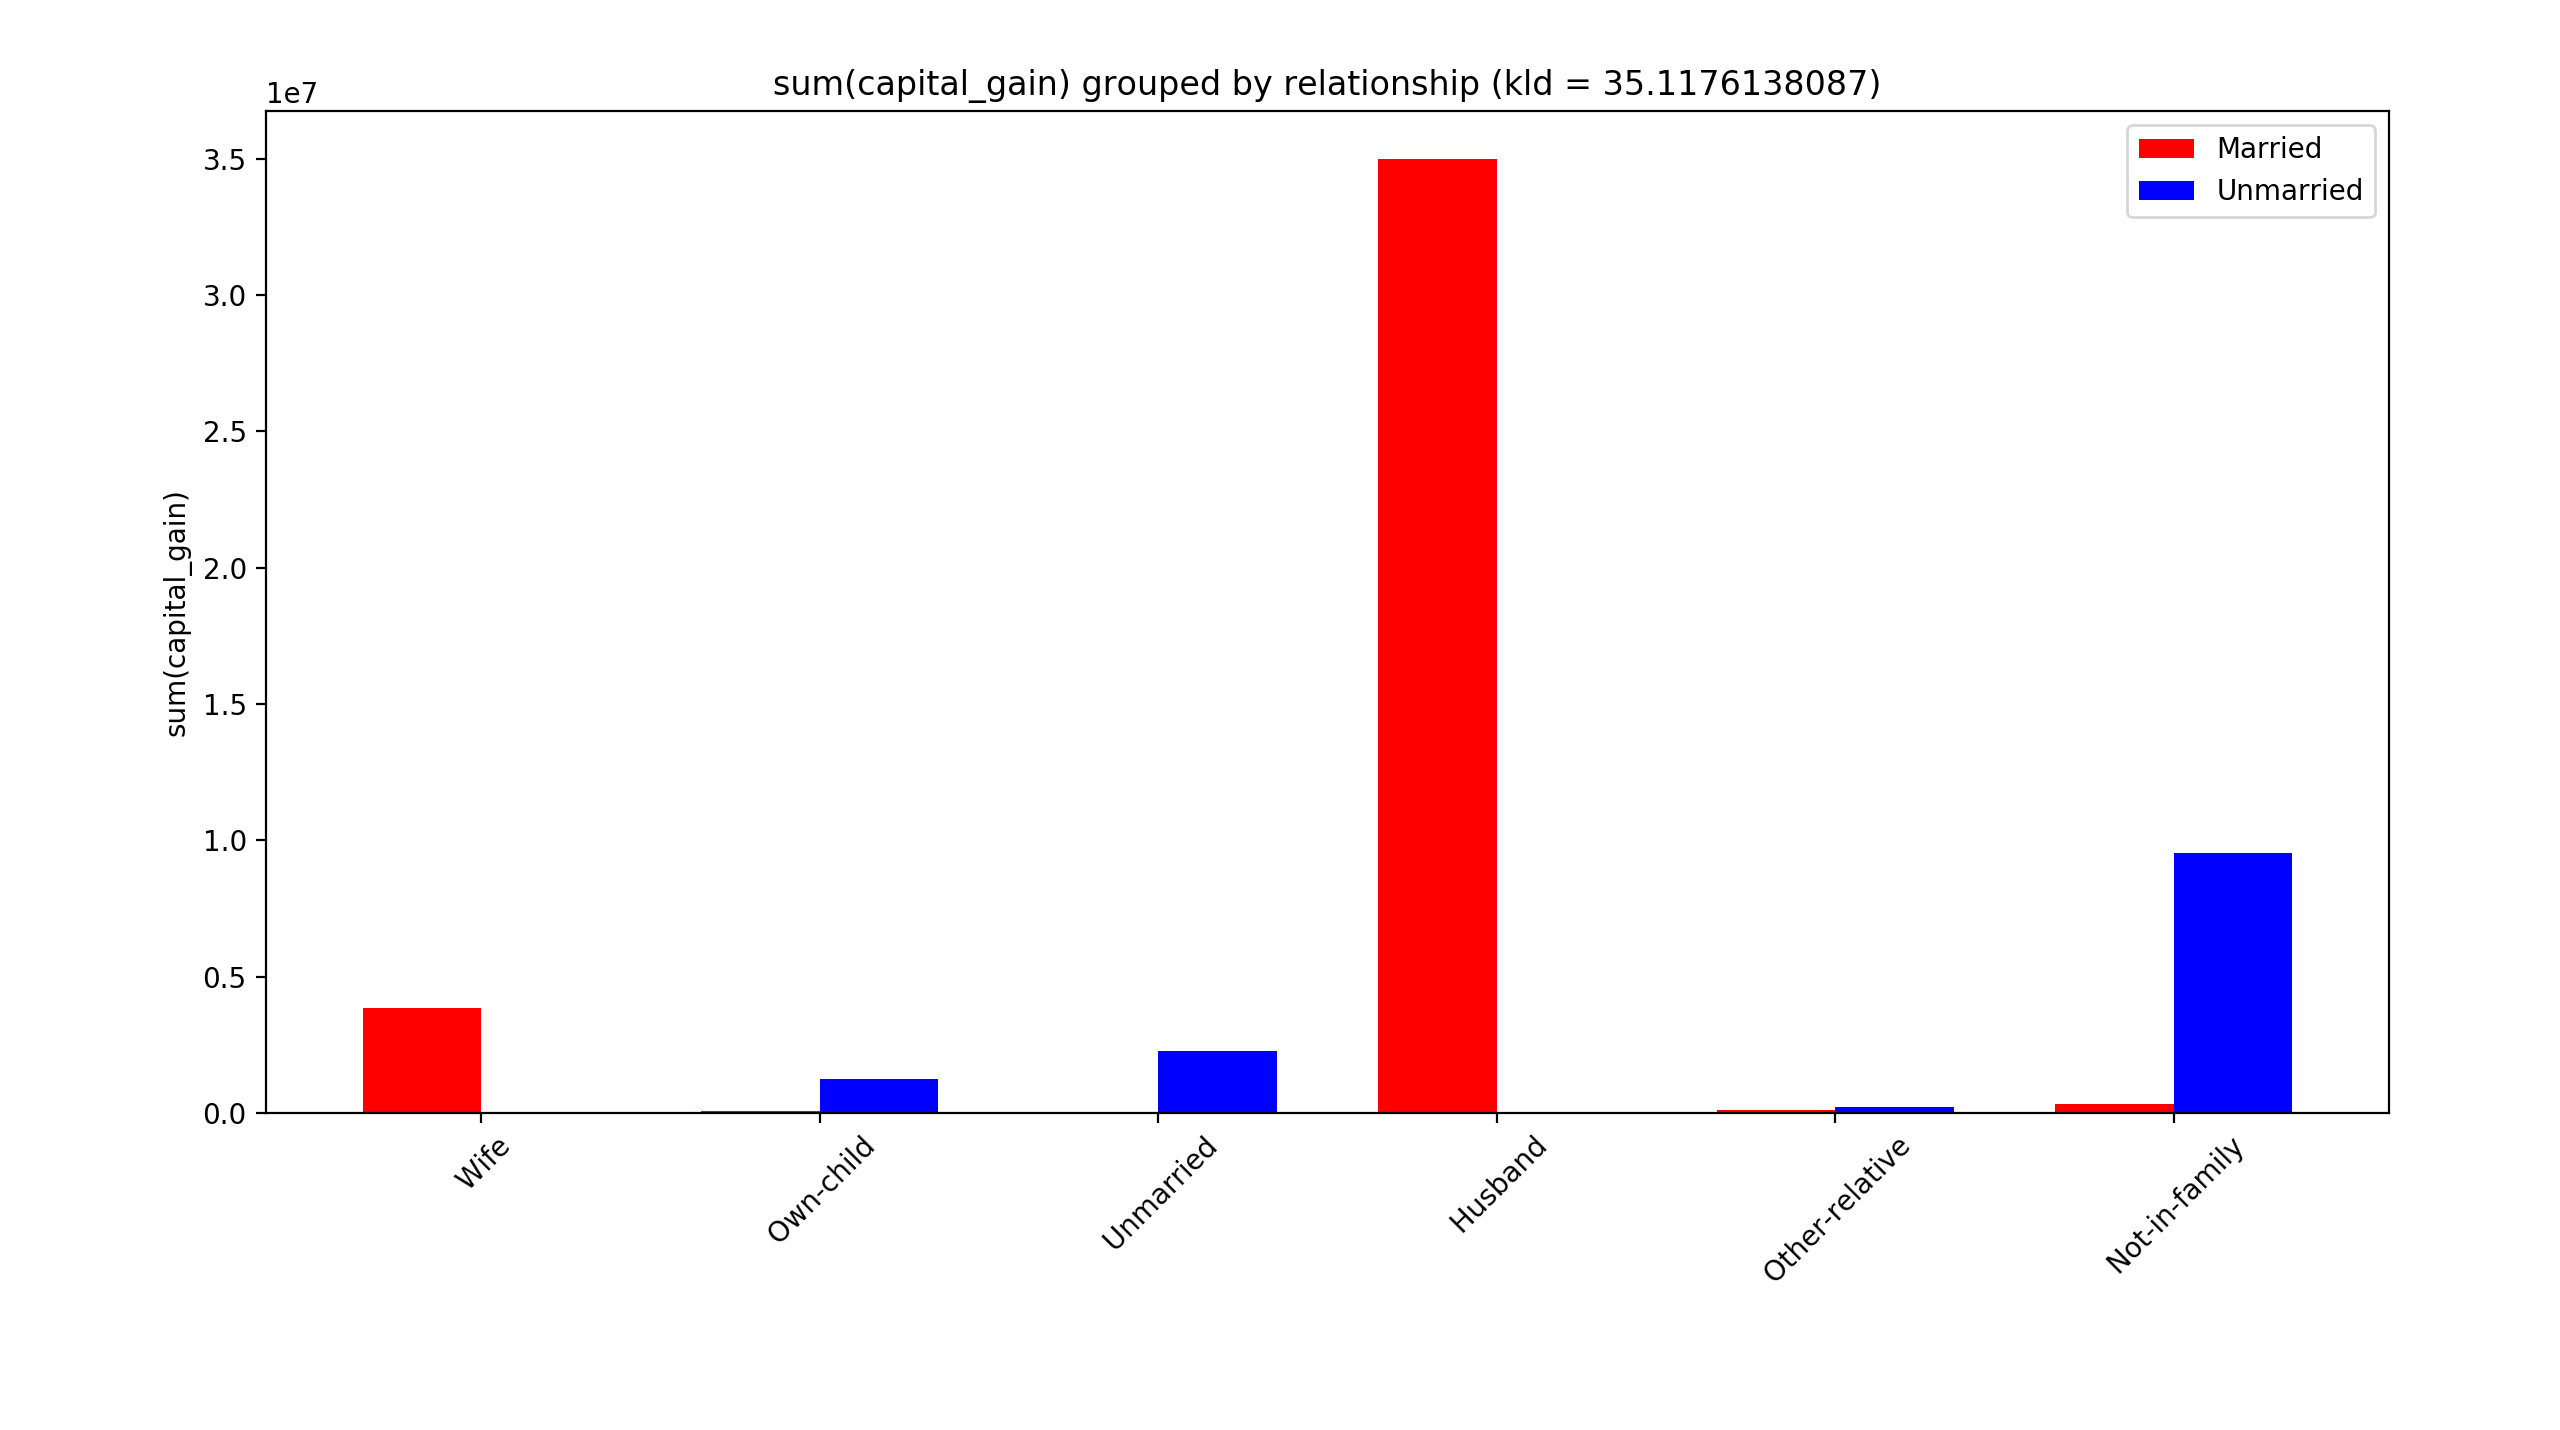
\includegraphics[scale=0.35]{figures/1relationship_sum_capital_gain_kld.png}
\end{figure}

\begin{figure}[h]
	\centering
	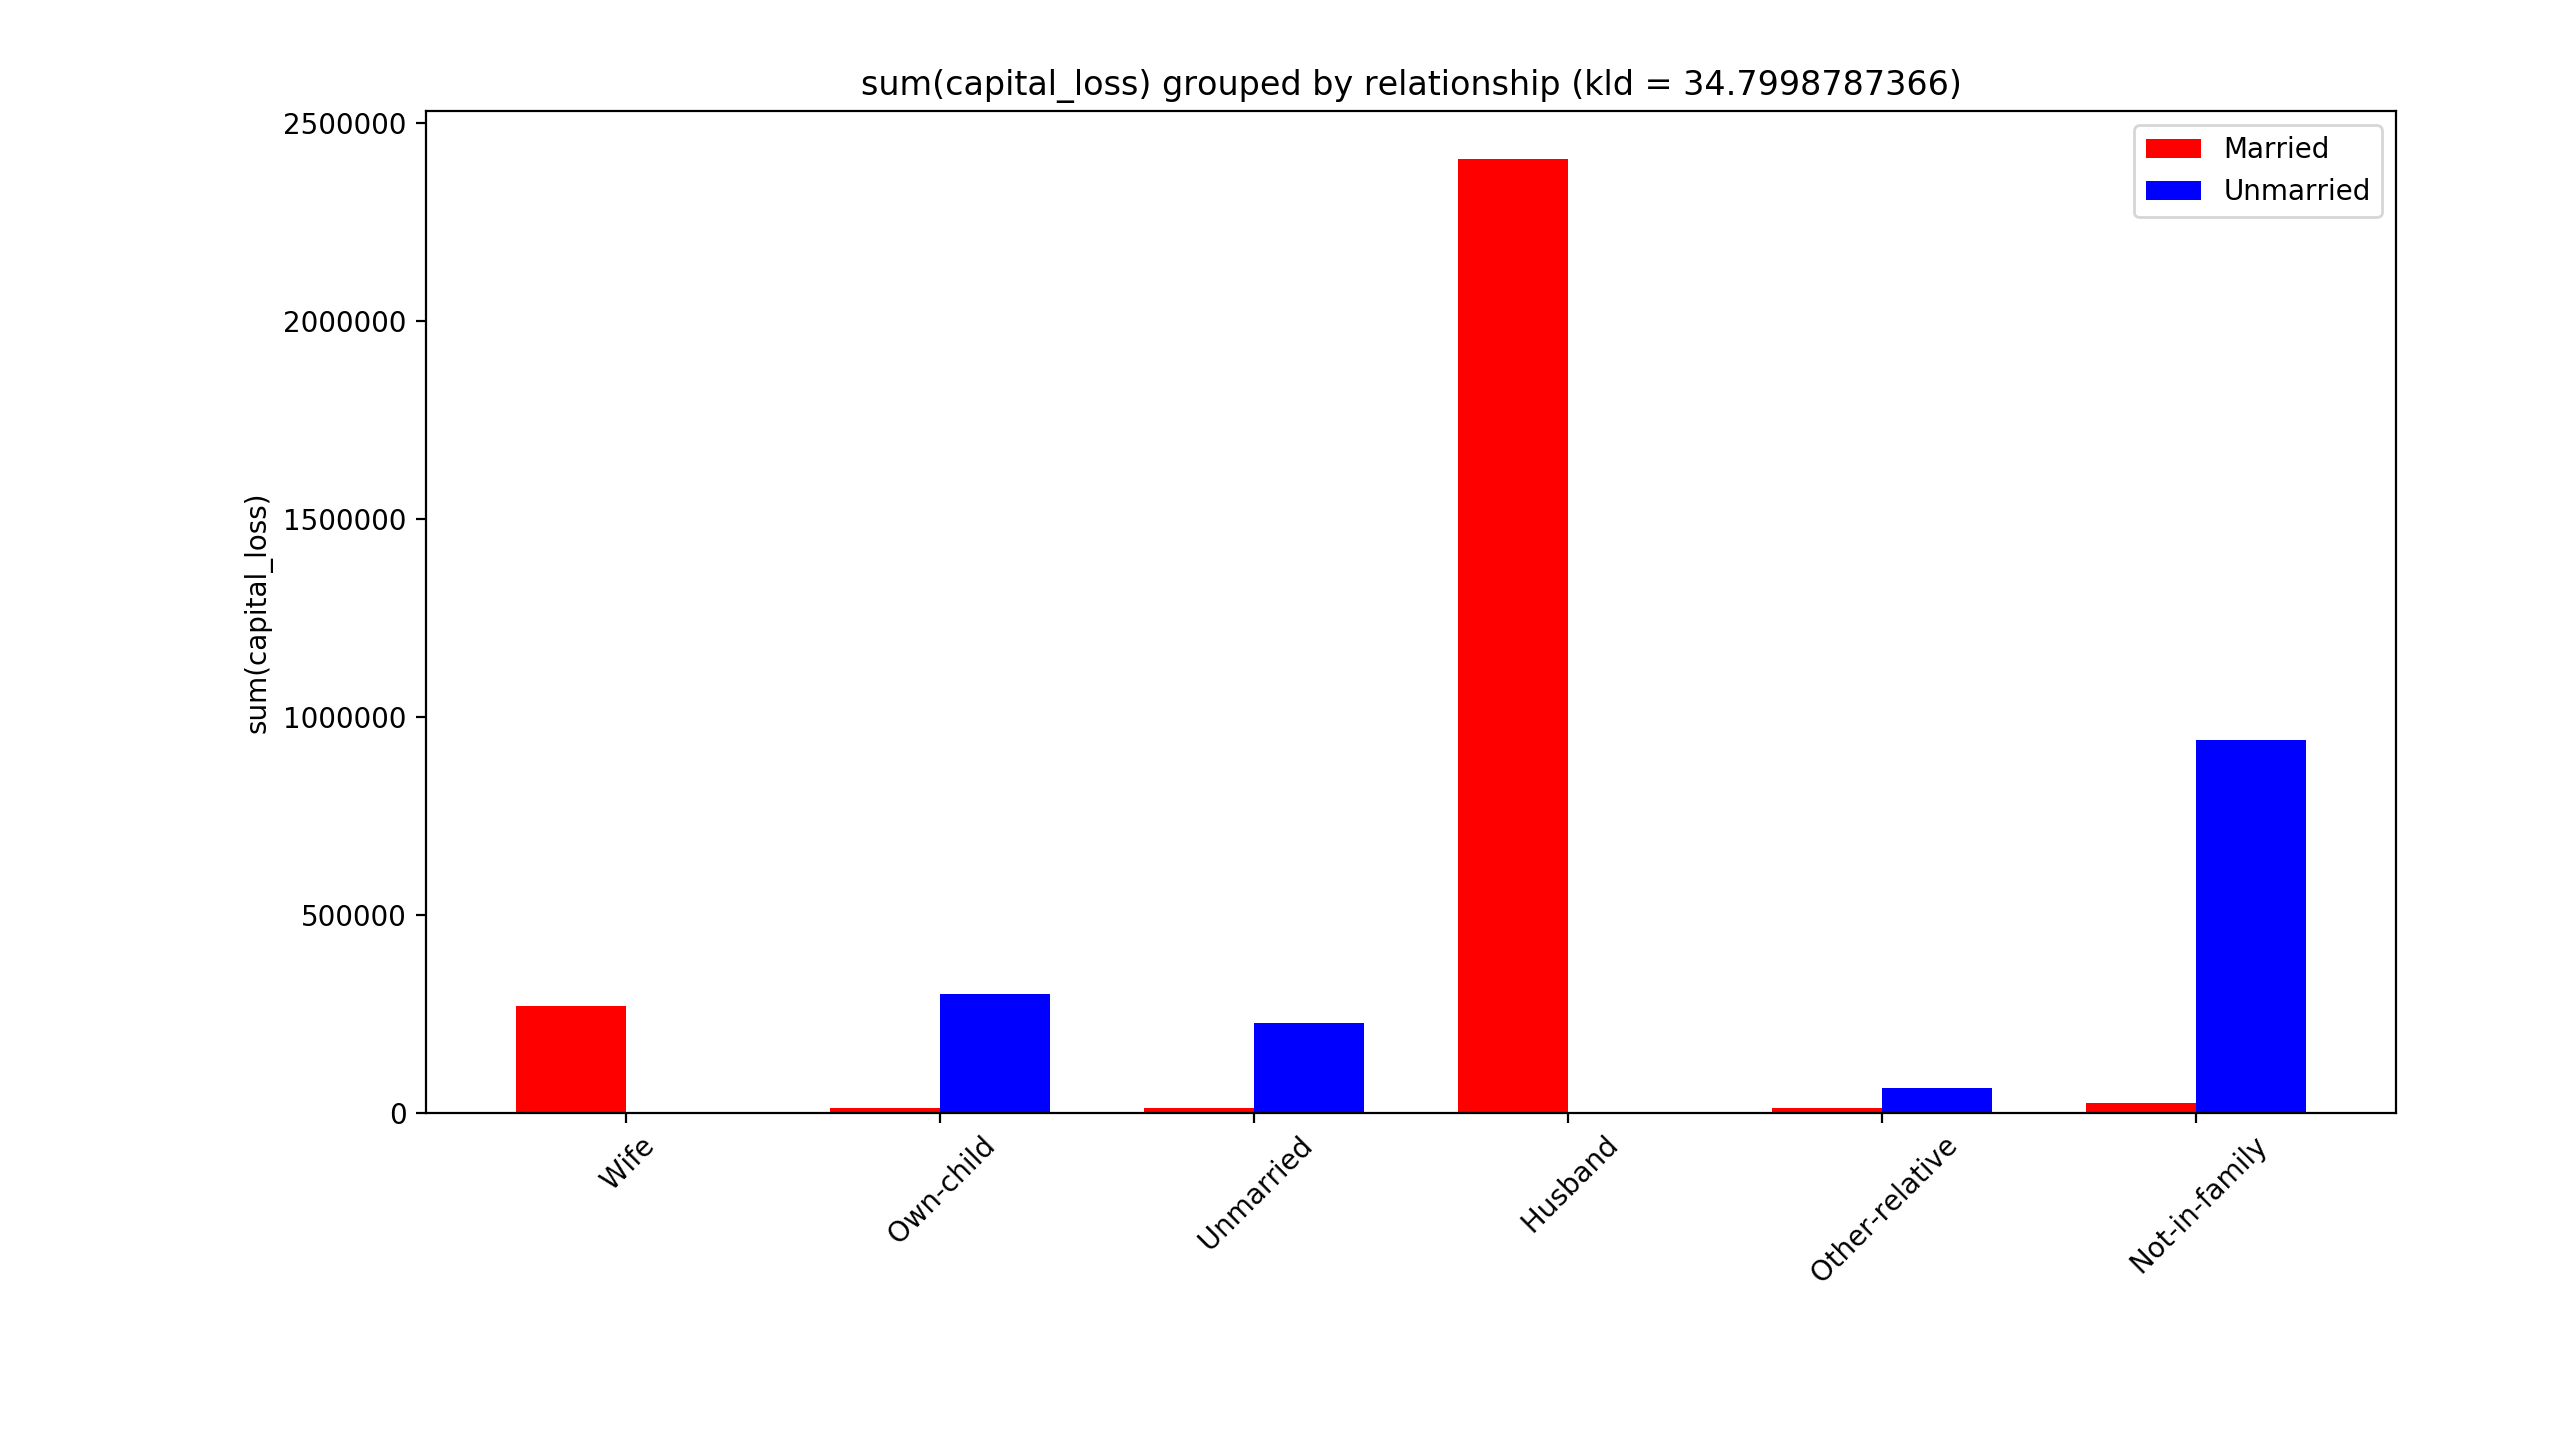
\includegraphics[scale=0.35]{figures/2relationship_sum_captial_loss_kld.png}
\end{figure}

\begin{figure}[h]
	\centering
	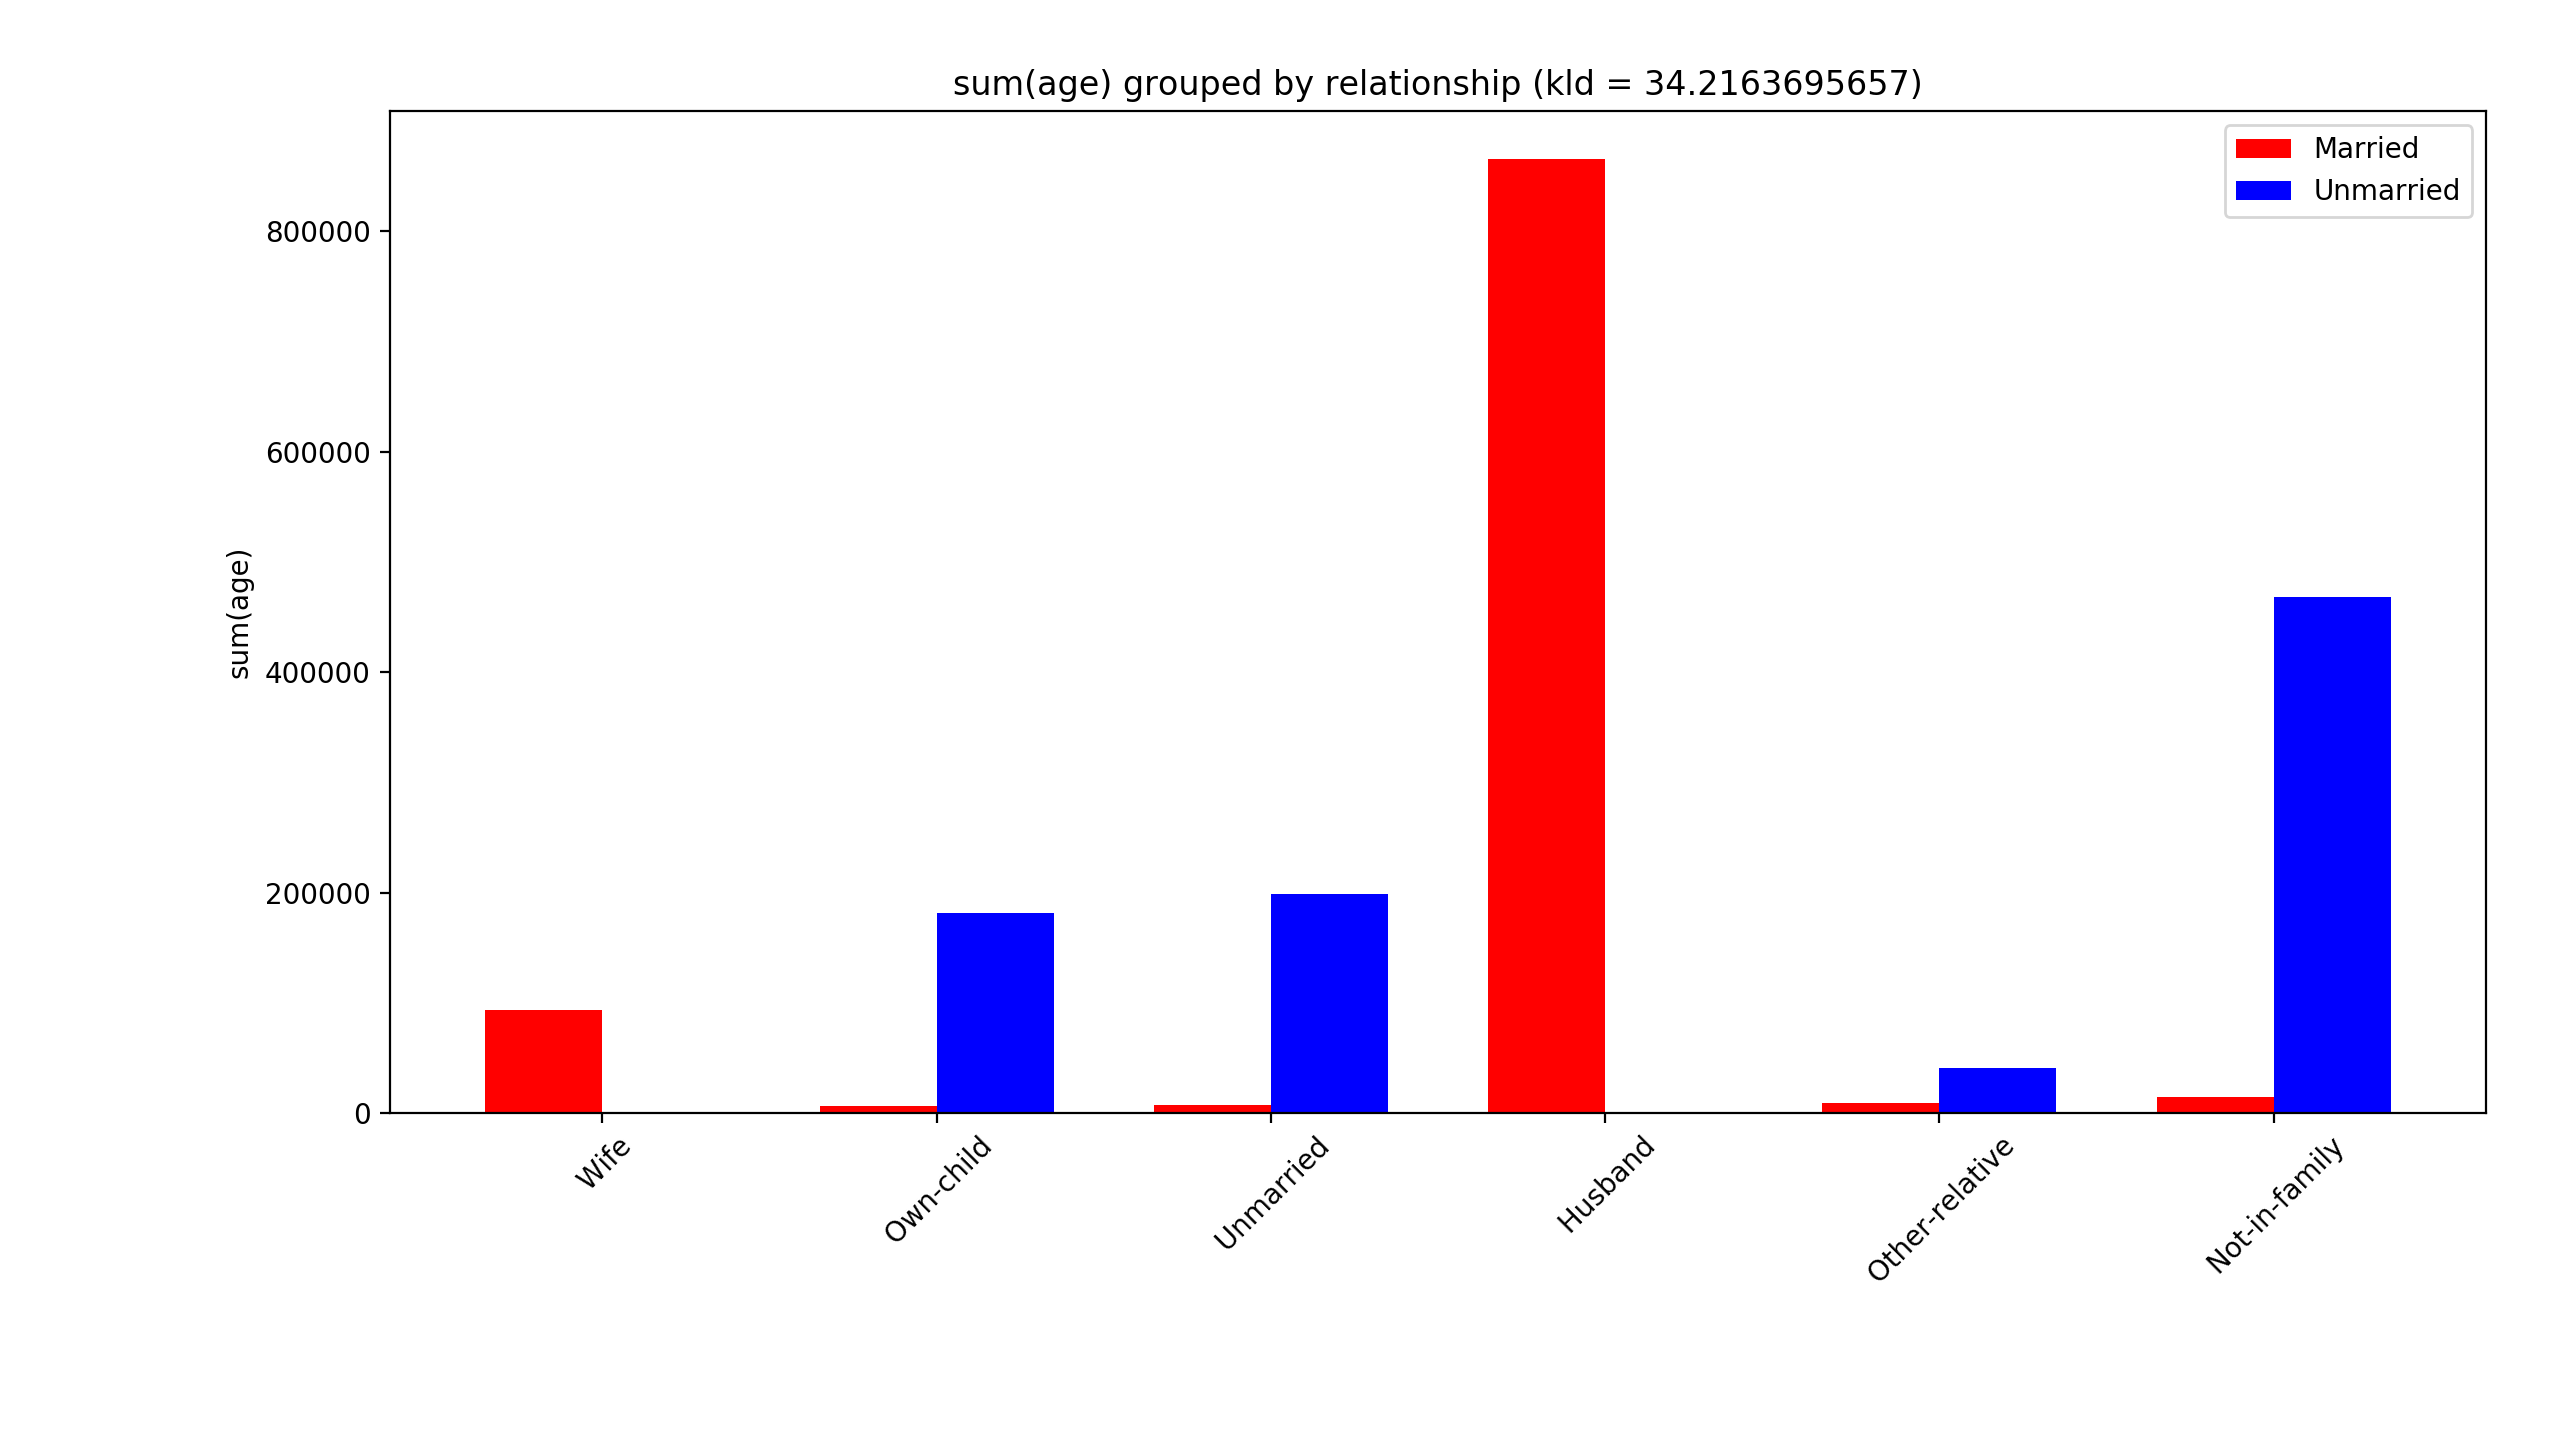
\includegraphics[scale=0.35]{figures/3relationship_sum_age_kld.png}
\end{figure}

\begin{figure}[h]
	\centering
	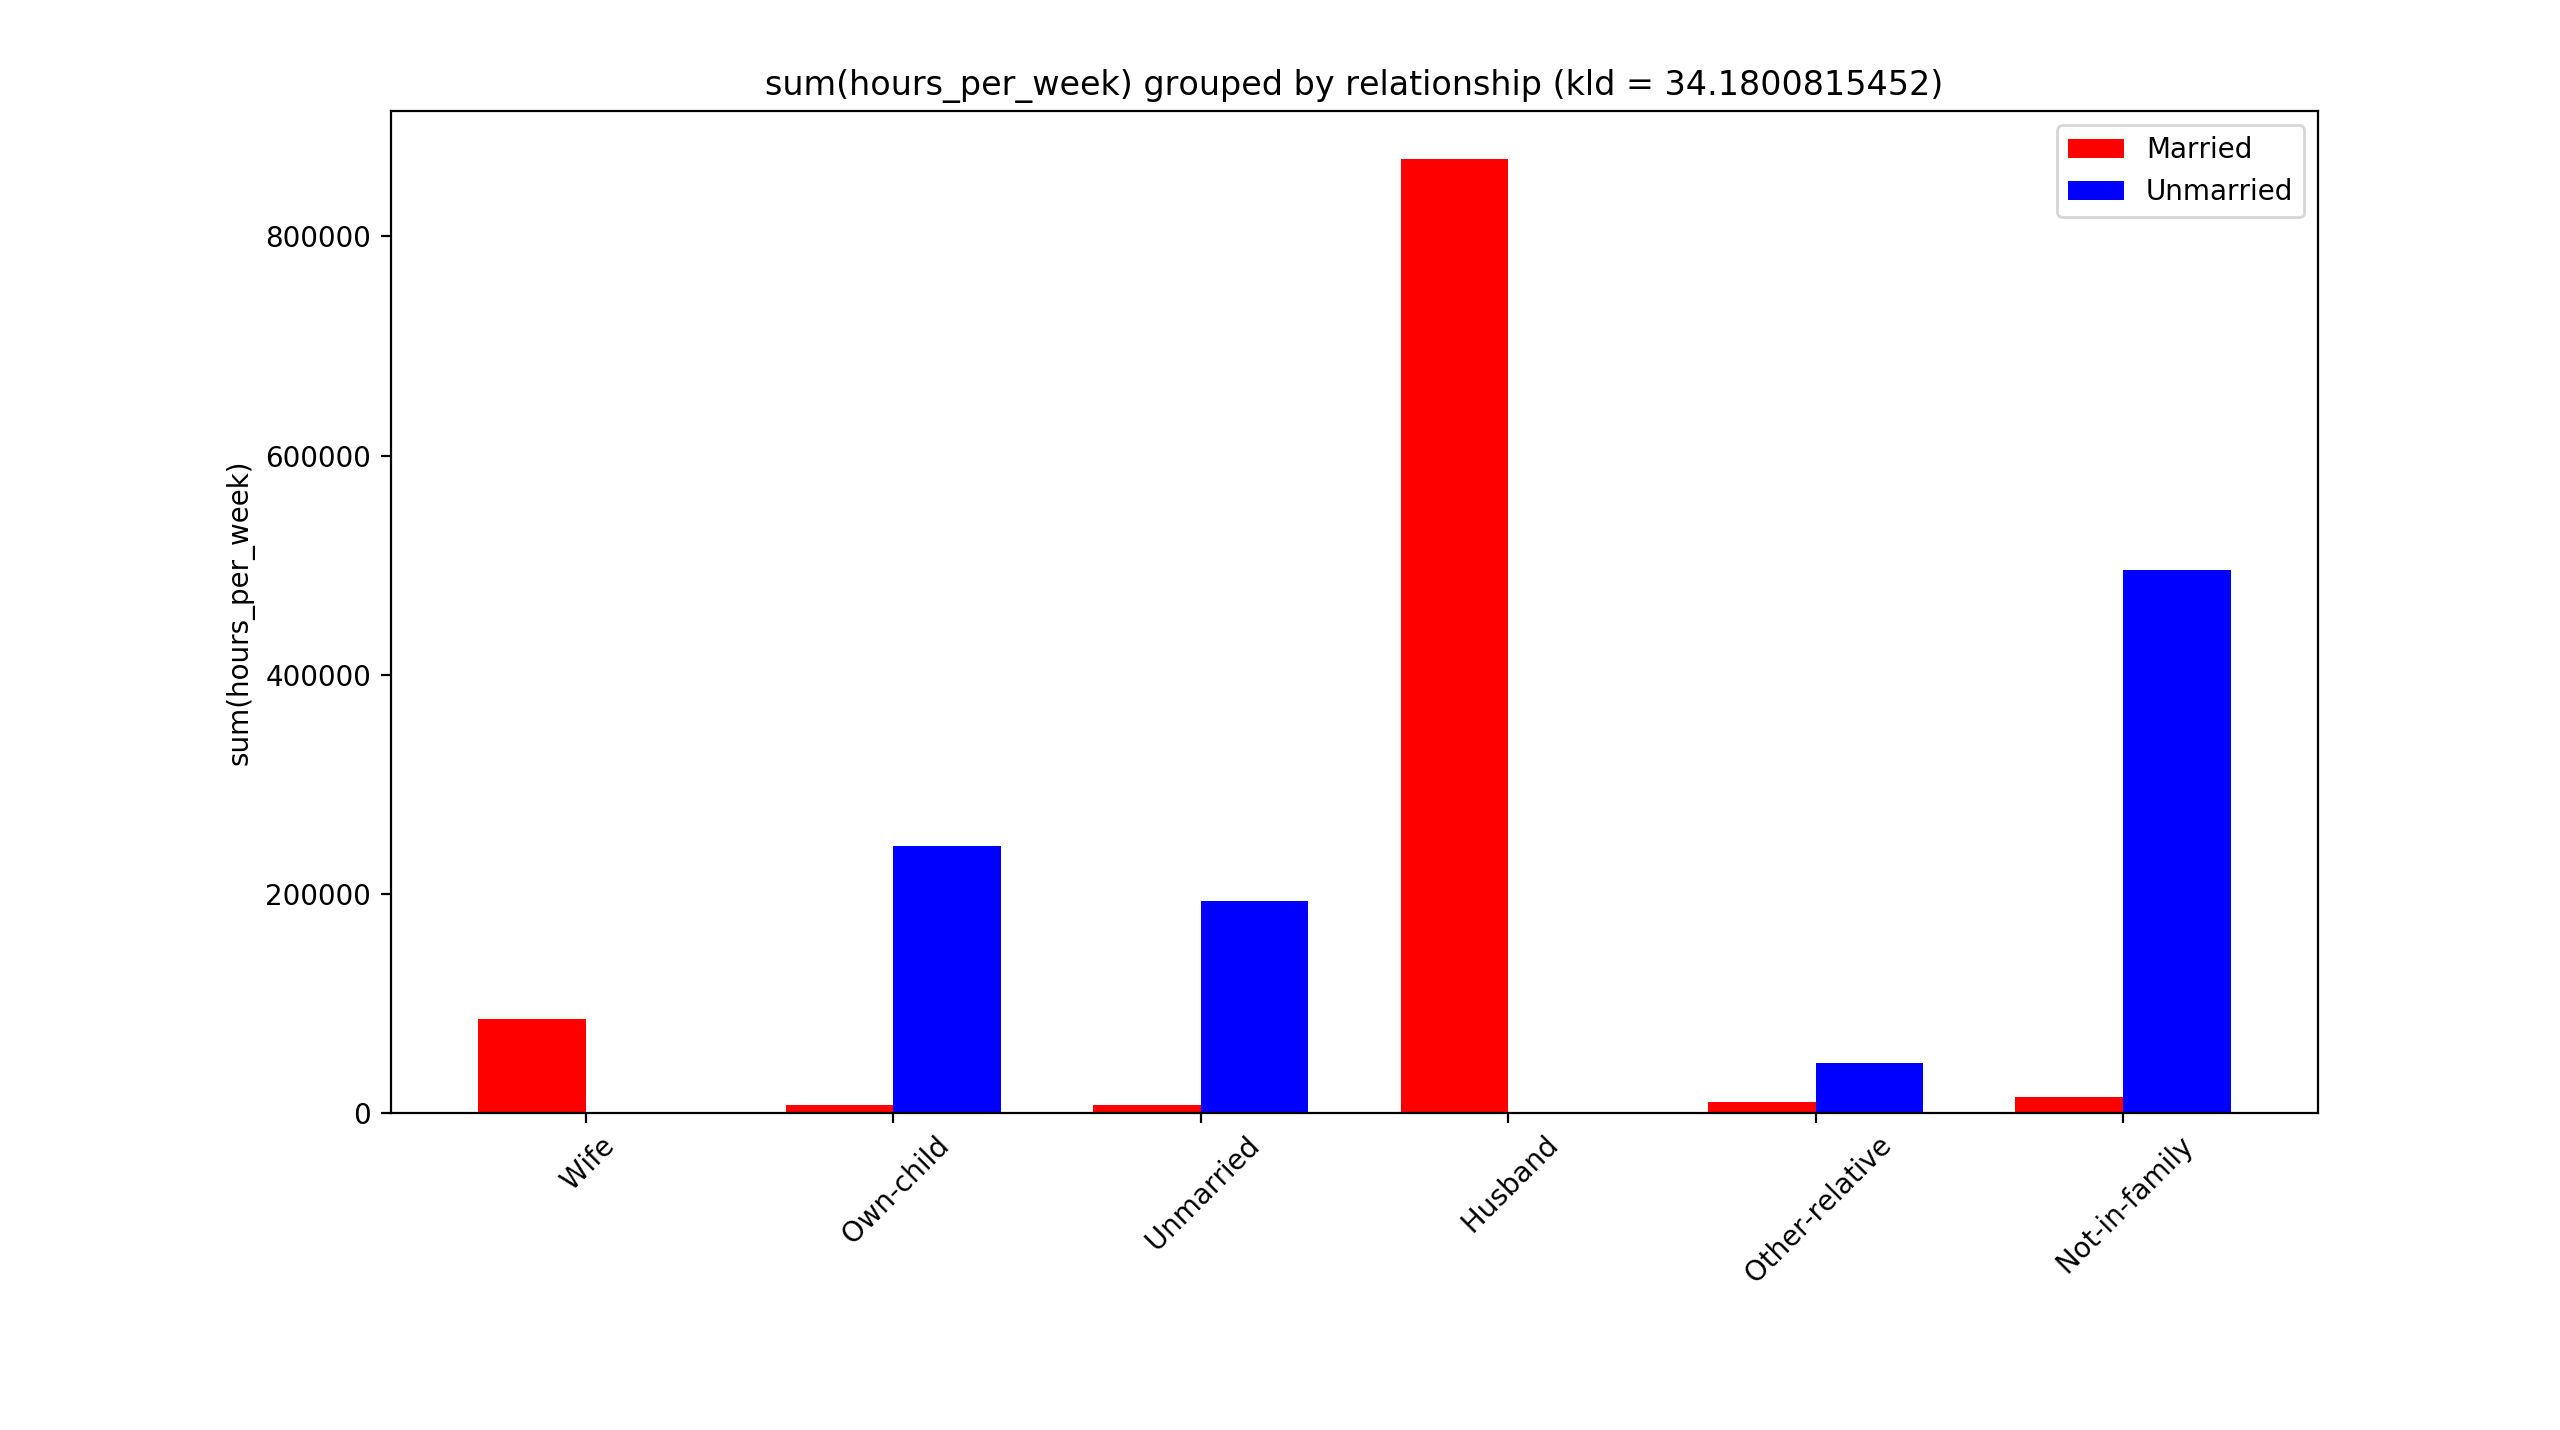
\includegraphics[scale=0.35]{figures/4relationship_sum_hours_per_week_kld.png}
\end{figure}

\begin{figure}[h]
	\centering
	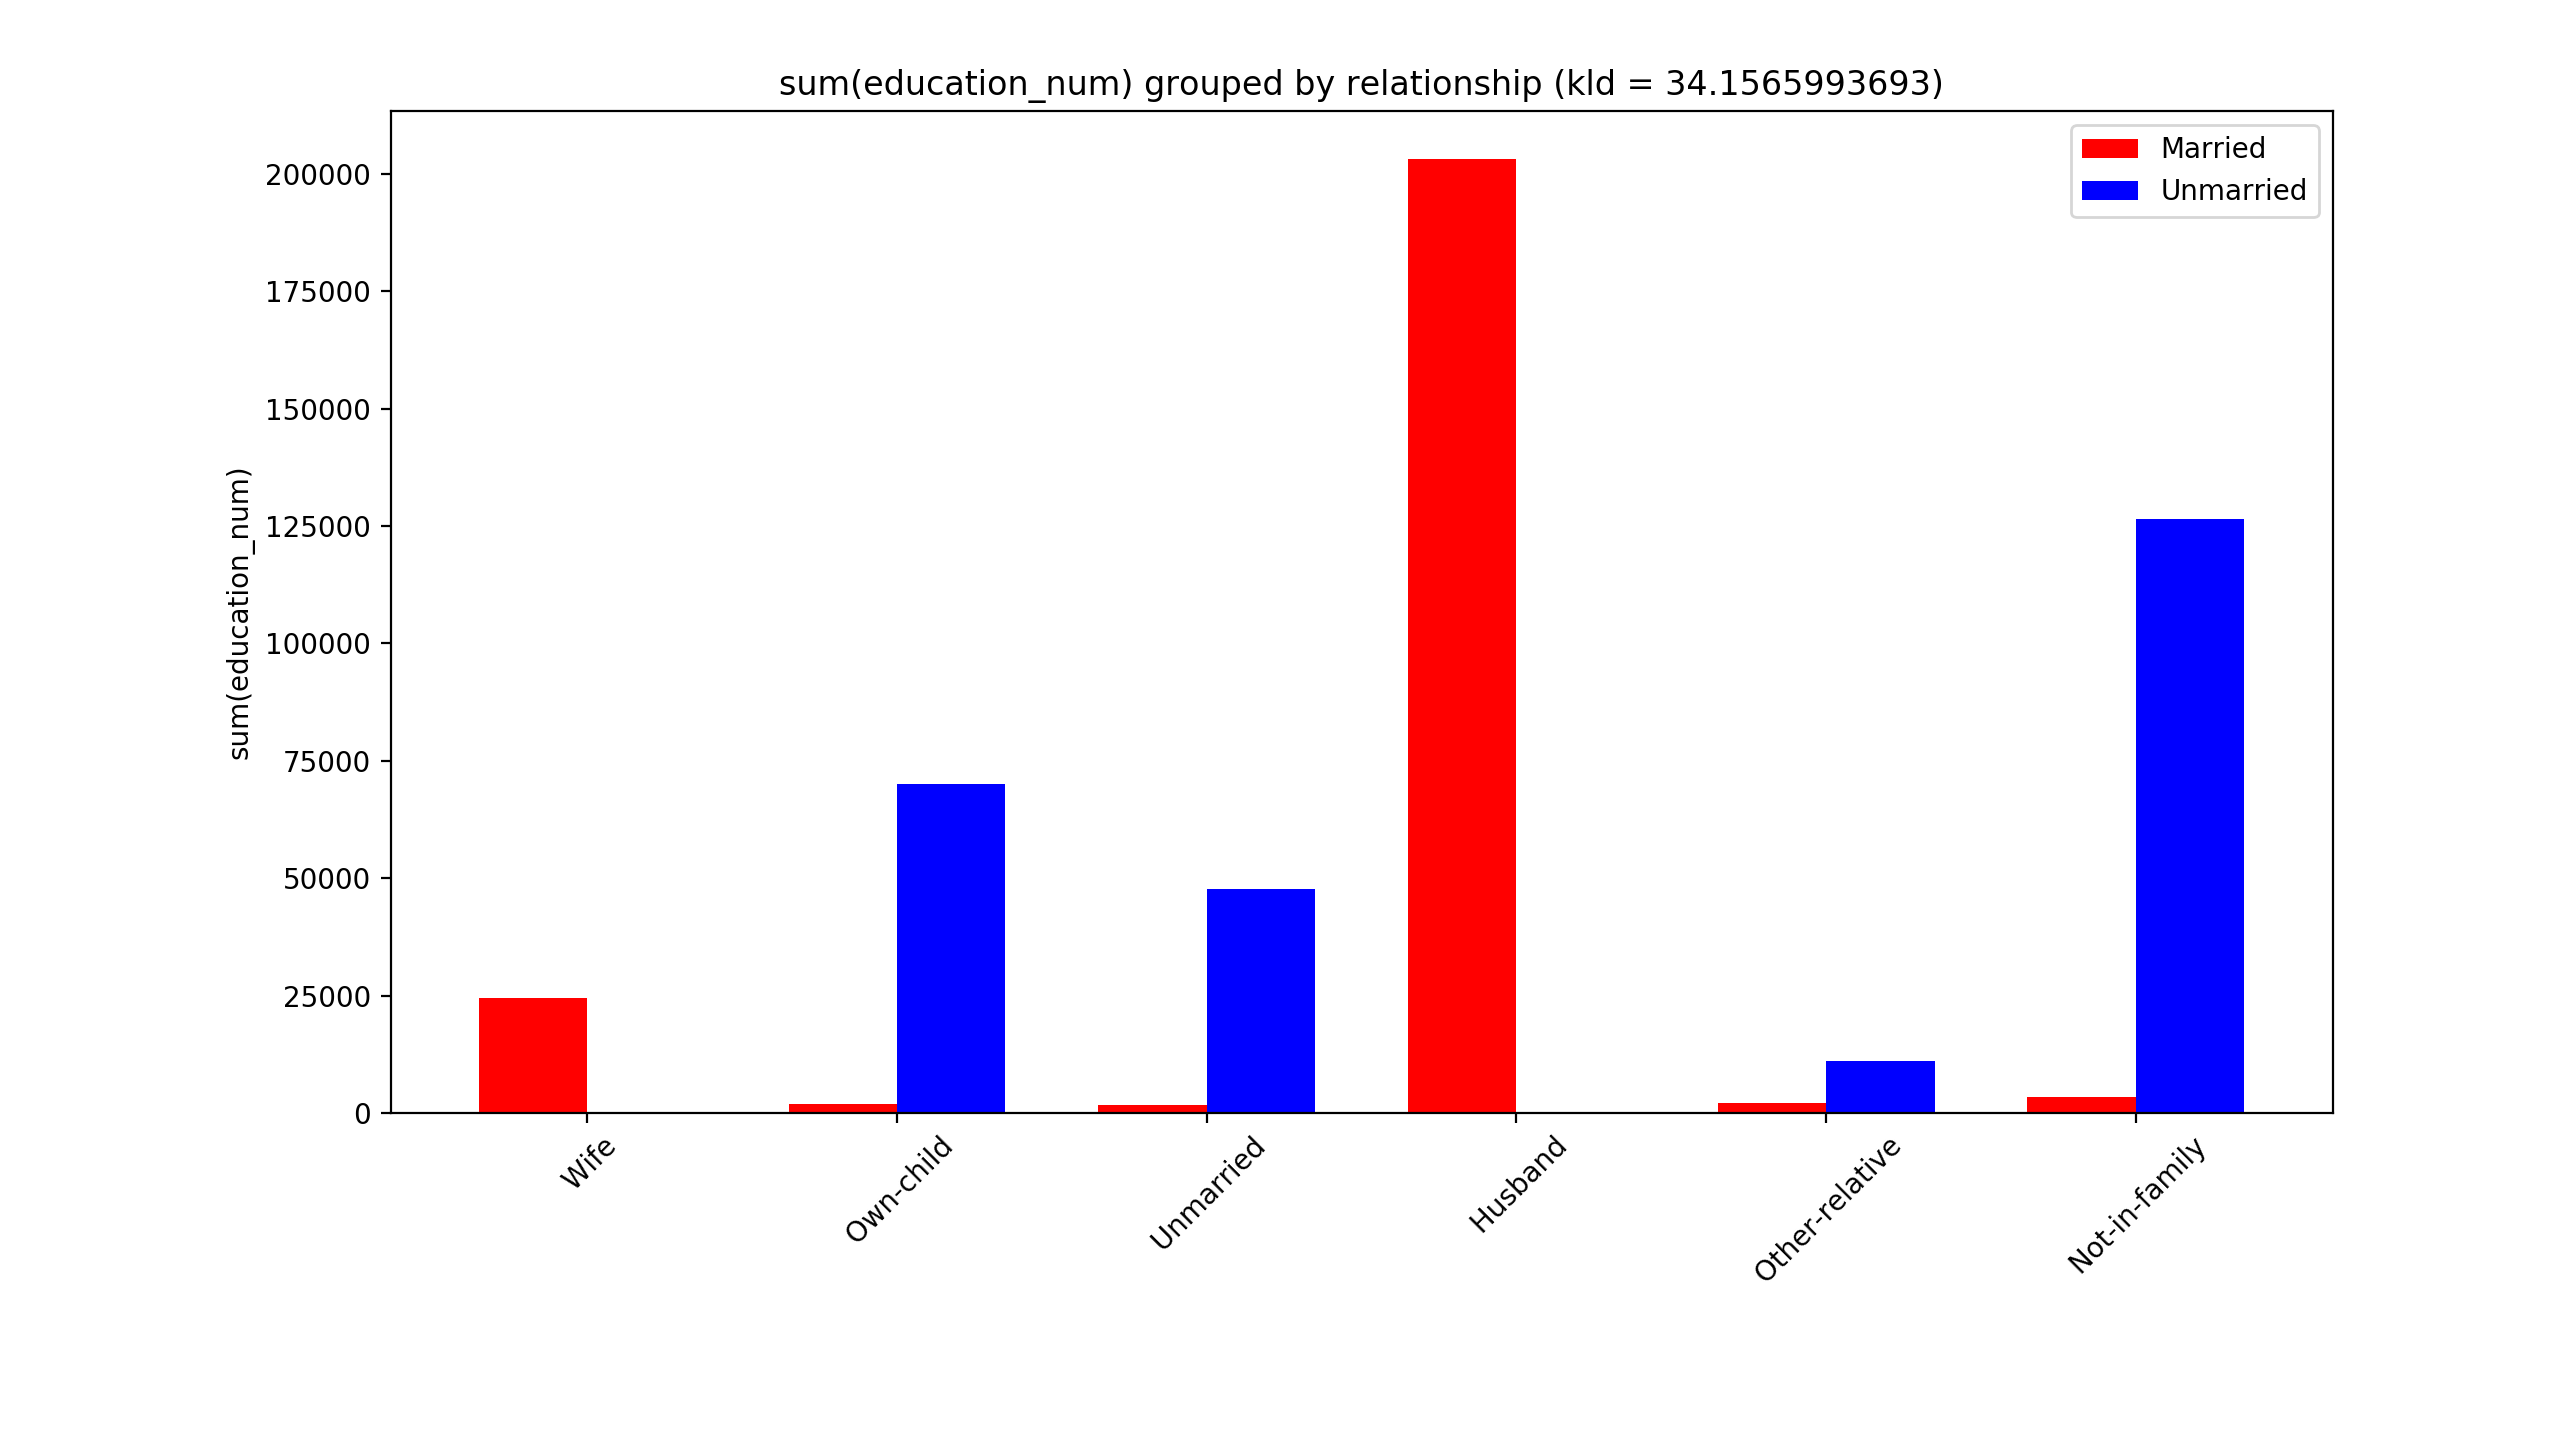
\includegraphics[scale=0.35]{figures/5relationship_sum_education_num_kld.png}
\end{figure}
\FloatBarrier

\subsubsection{Earth Mover's Distance}
The following are the visualizations of the most interesting queries returned when using Earth Mover's Distance.

\begin{figure}[h]
	\centering
	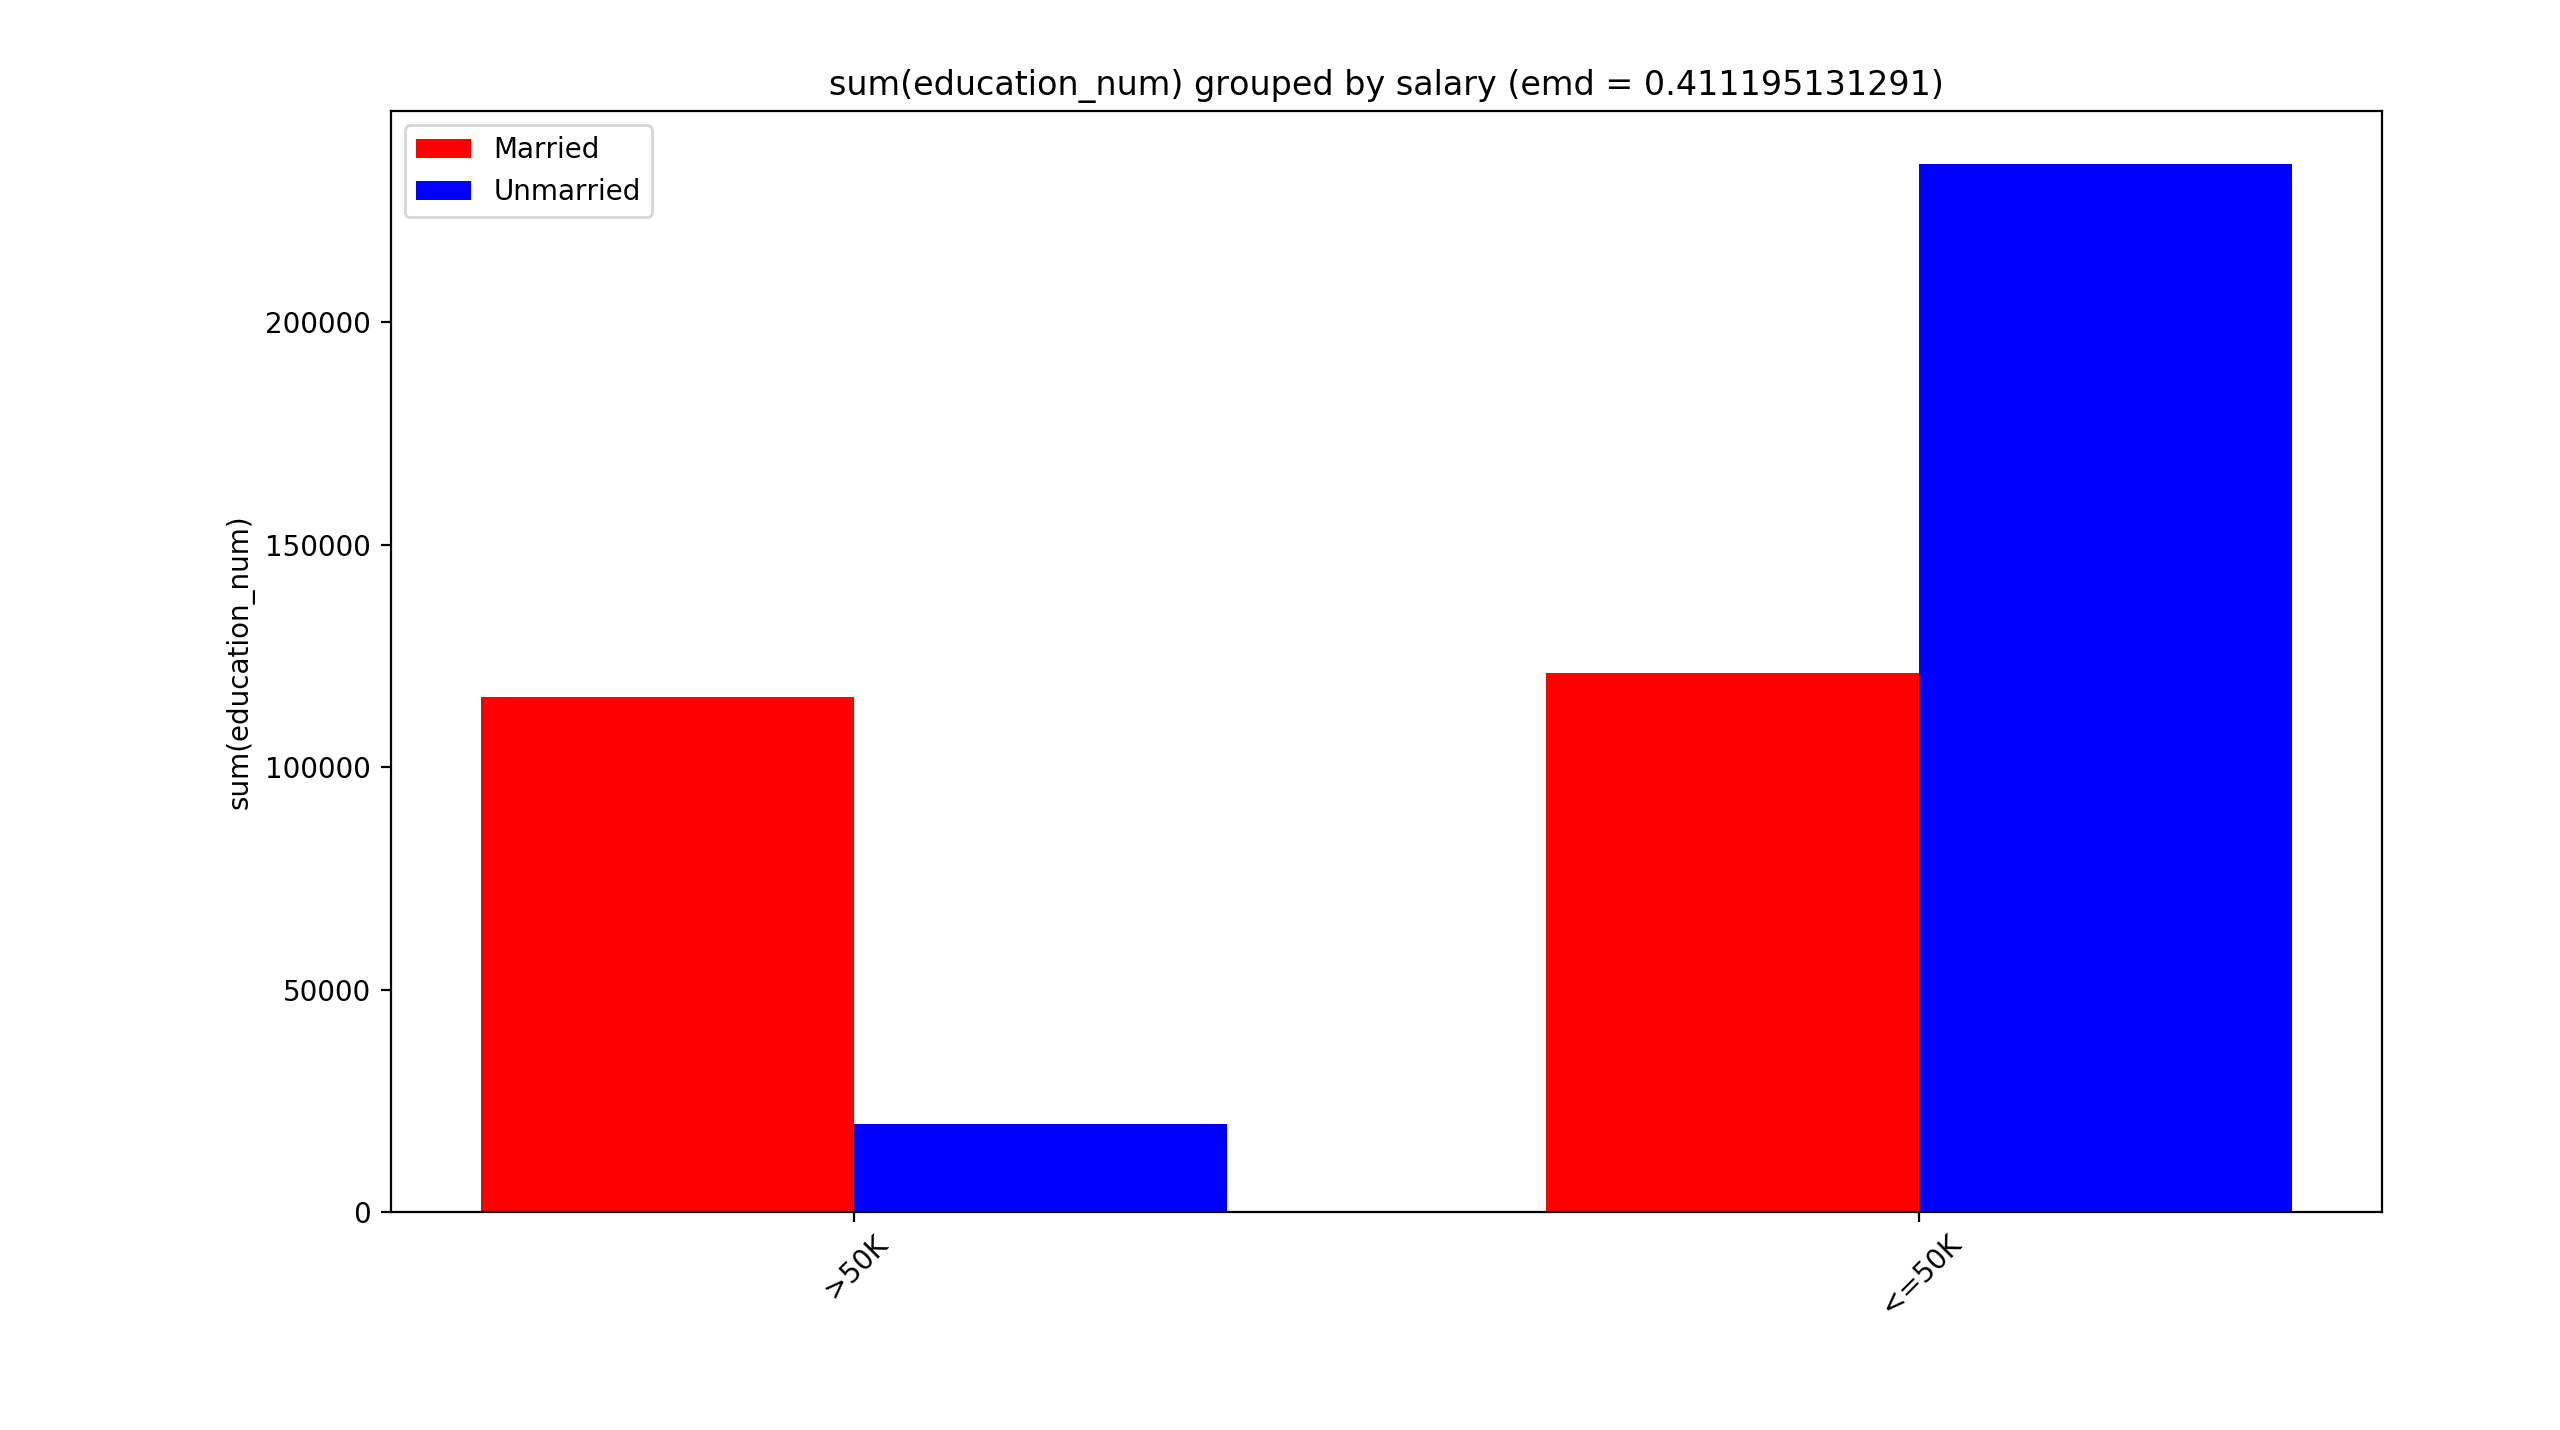
\includegraphics[scale=0.35]{figures/1salary_sum_education_num_emd.png}
\end{figure}

\begin{figure}[h]
	\centering
	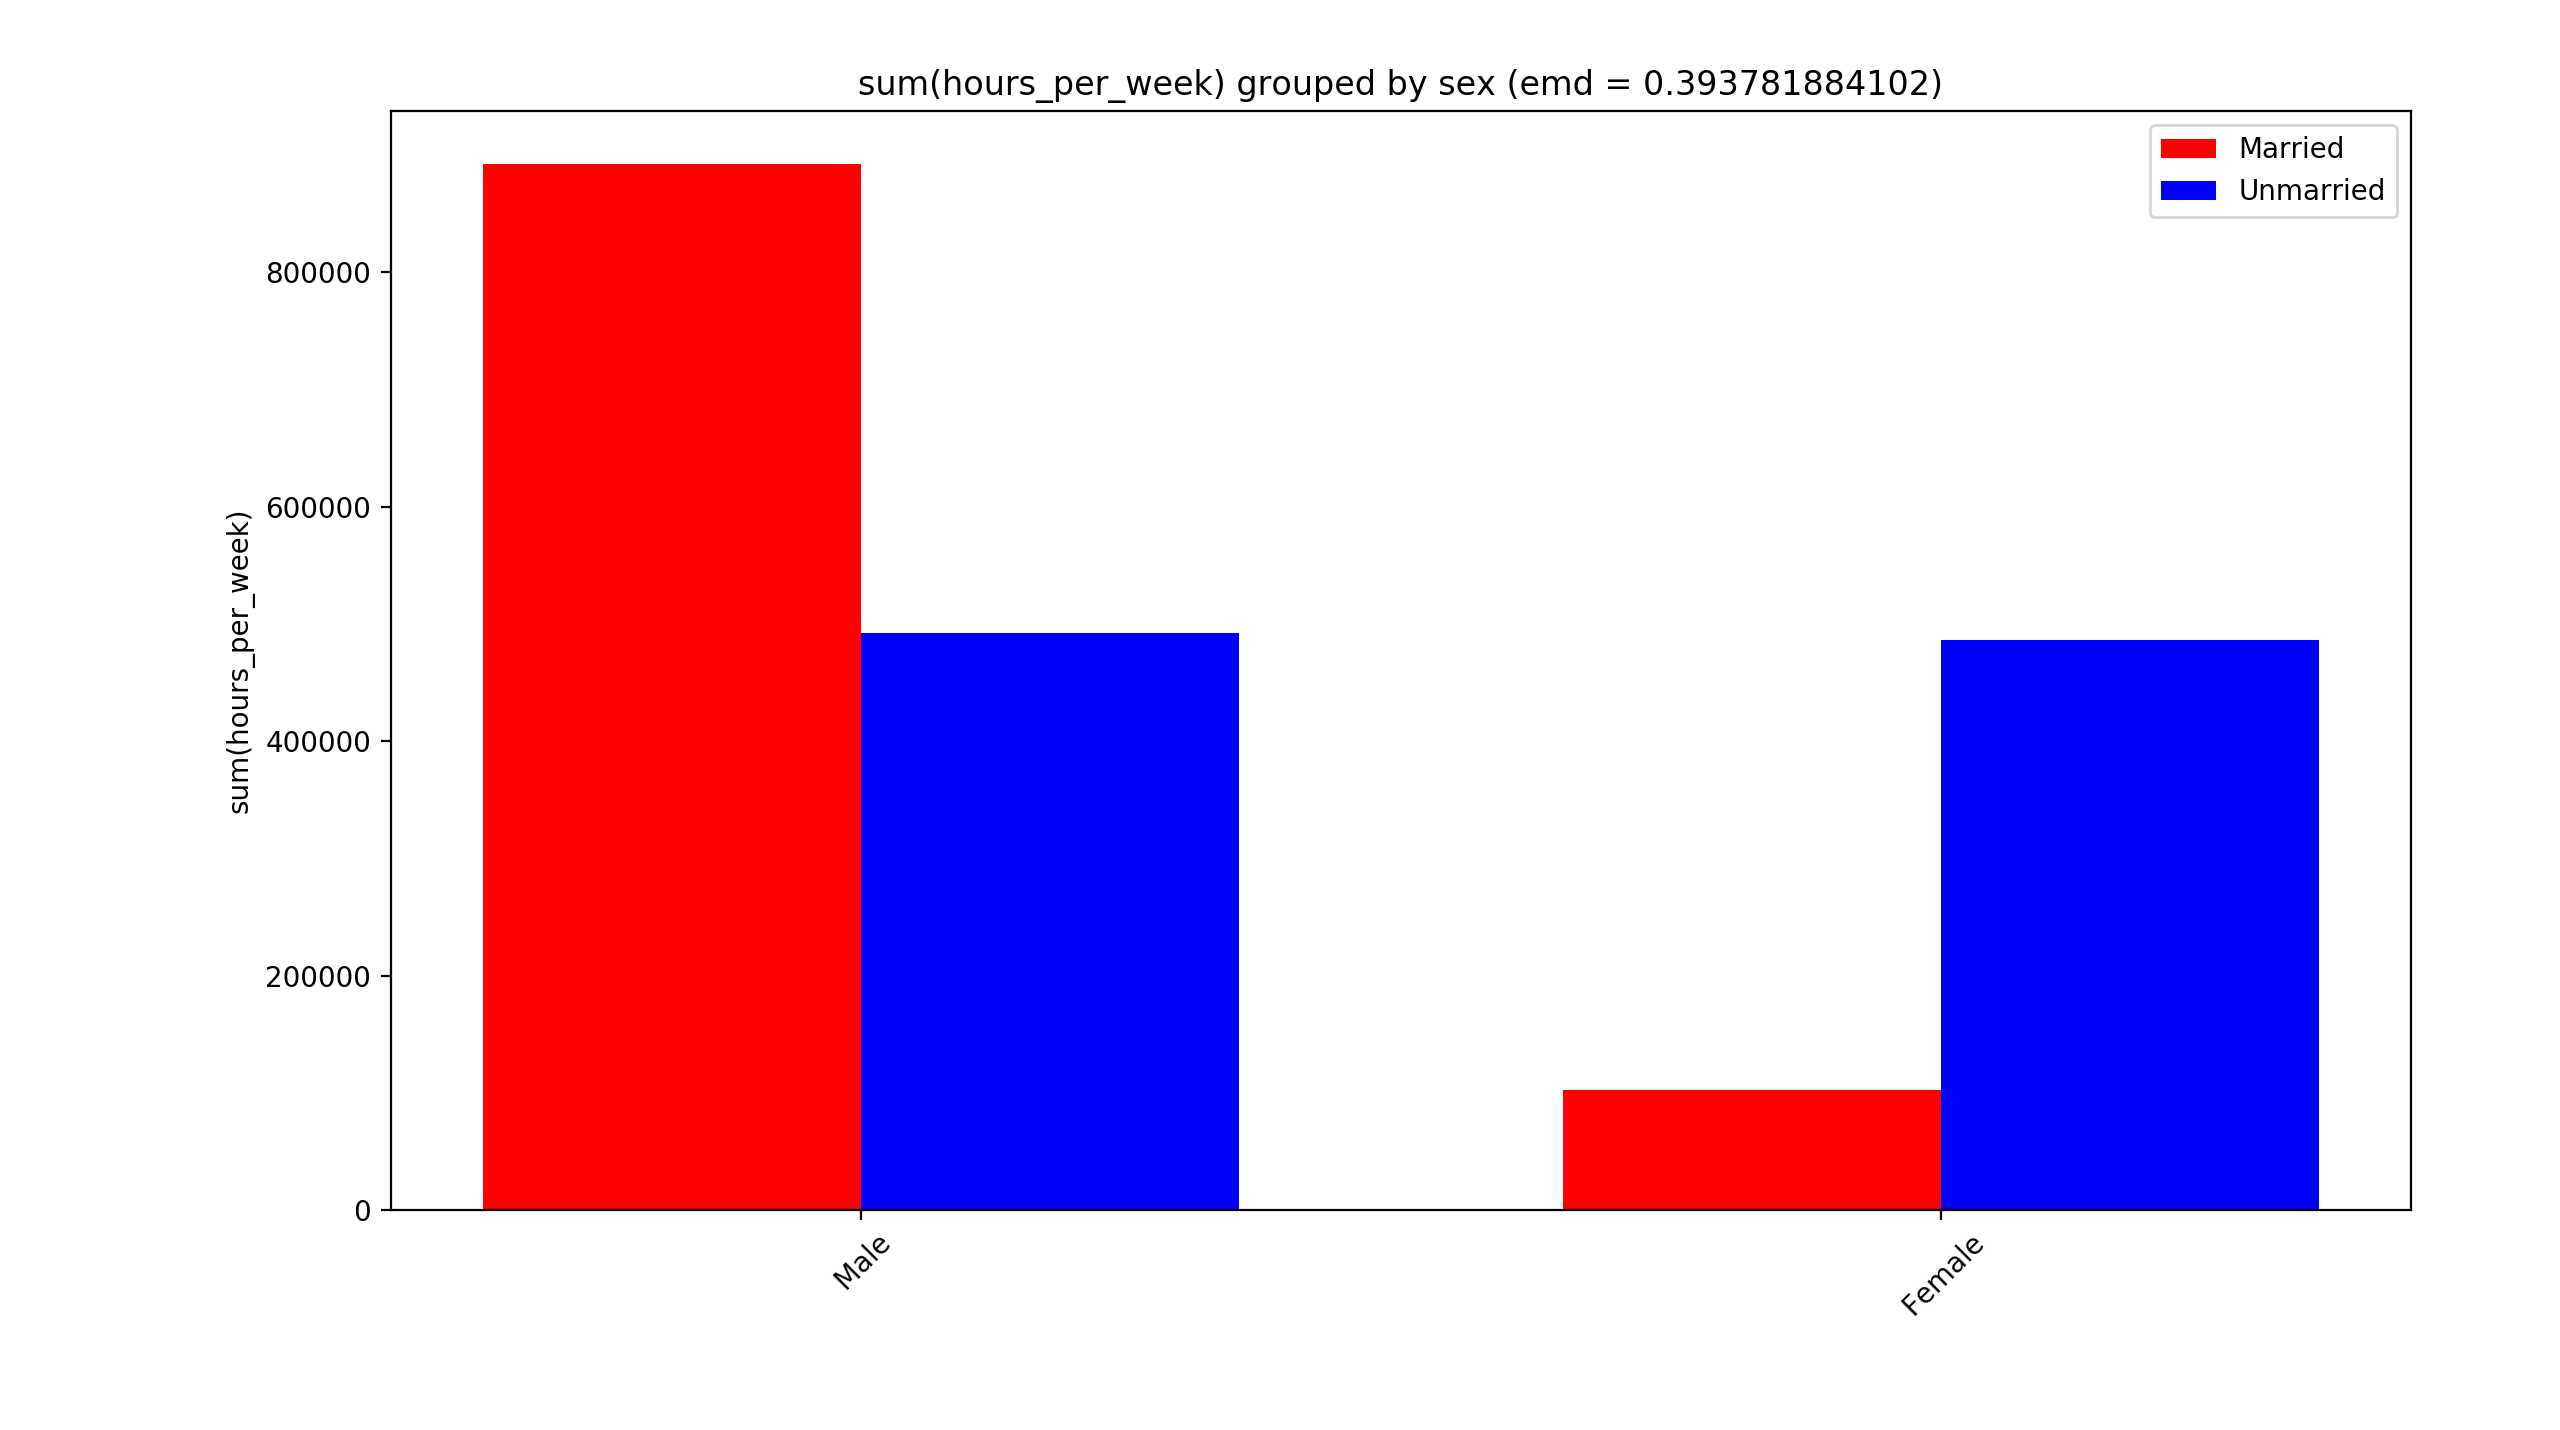
\includegraphics[scale=0.35]{figures/2sex_sum_hours_per_week_emd.png}
\end{figure}

\begin{figure}[h]
	\centering
	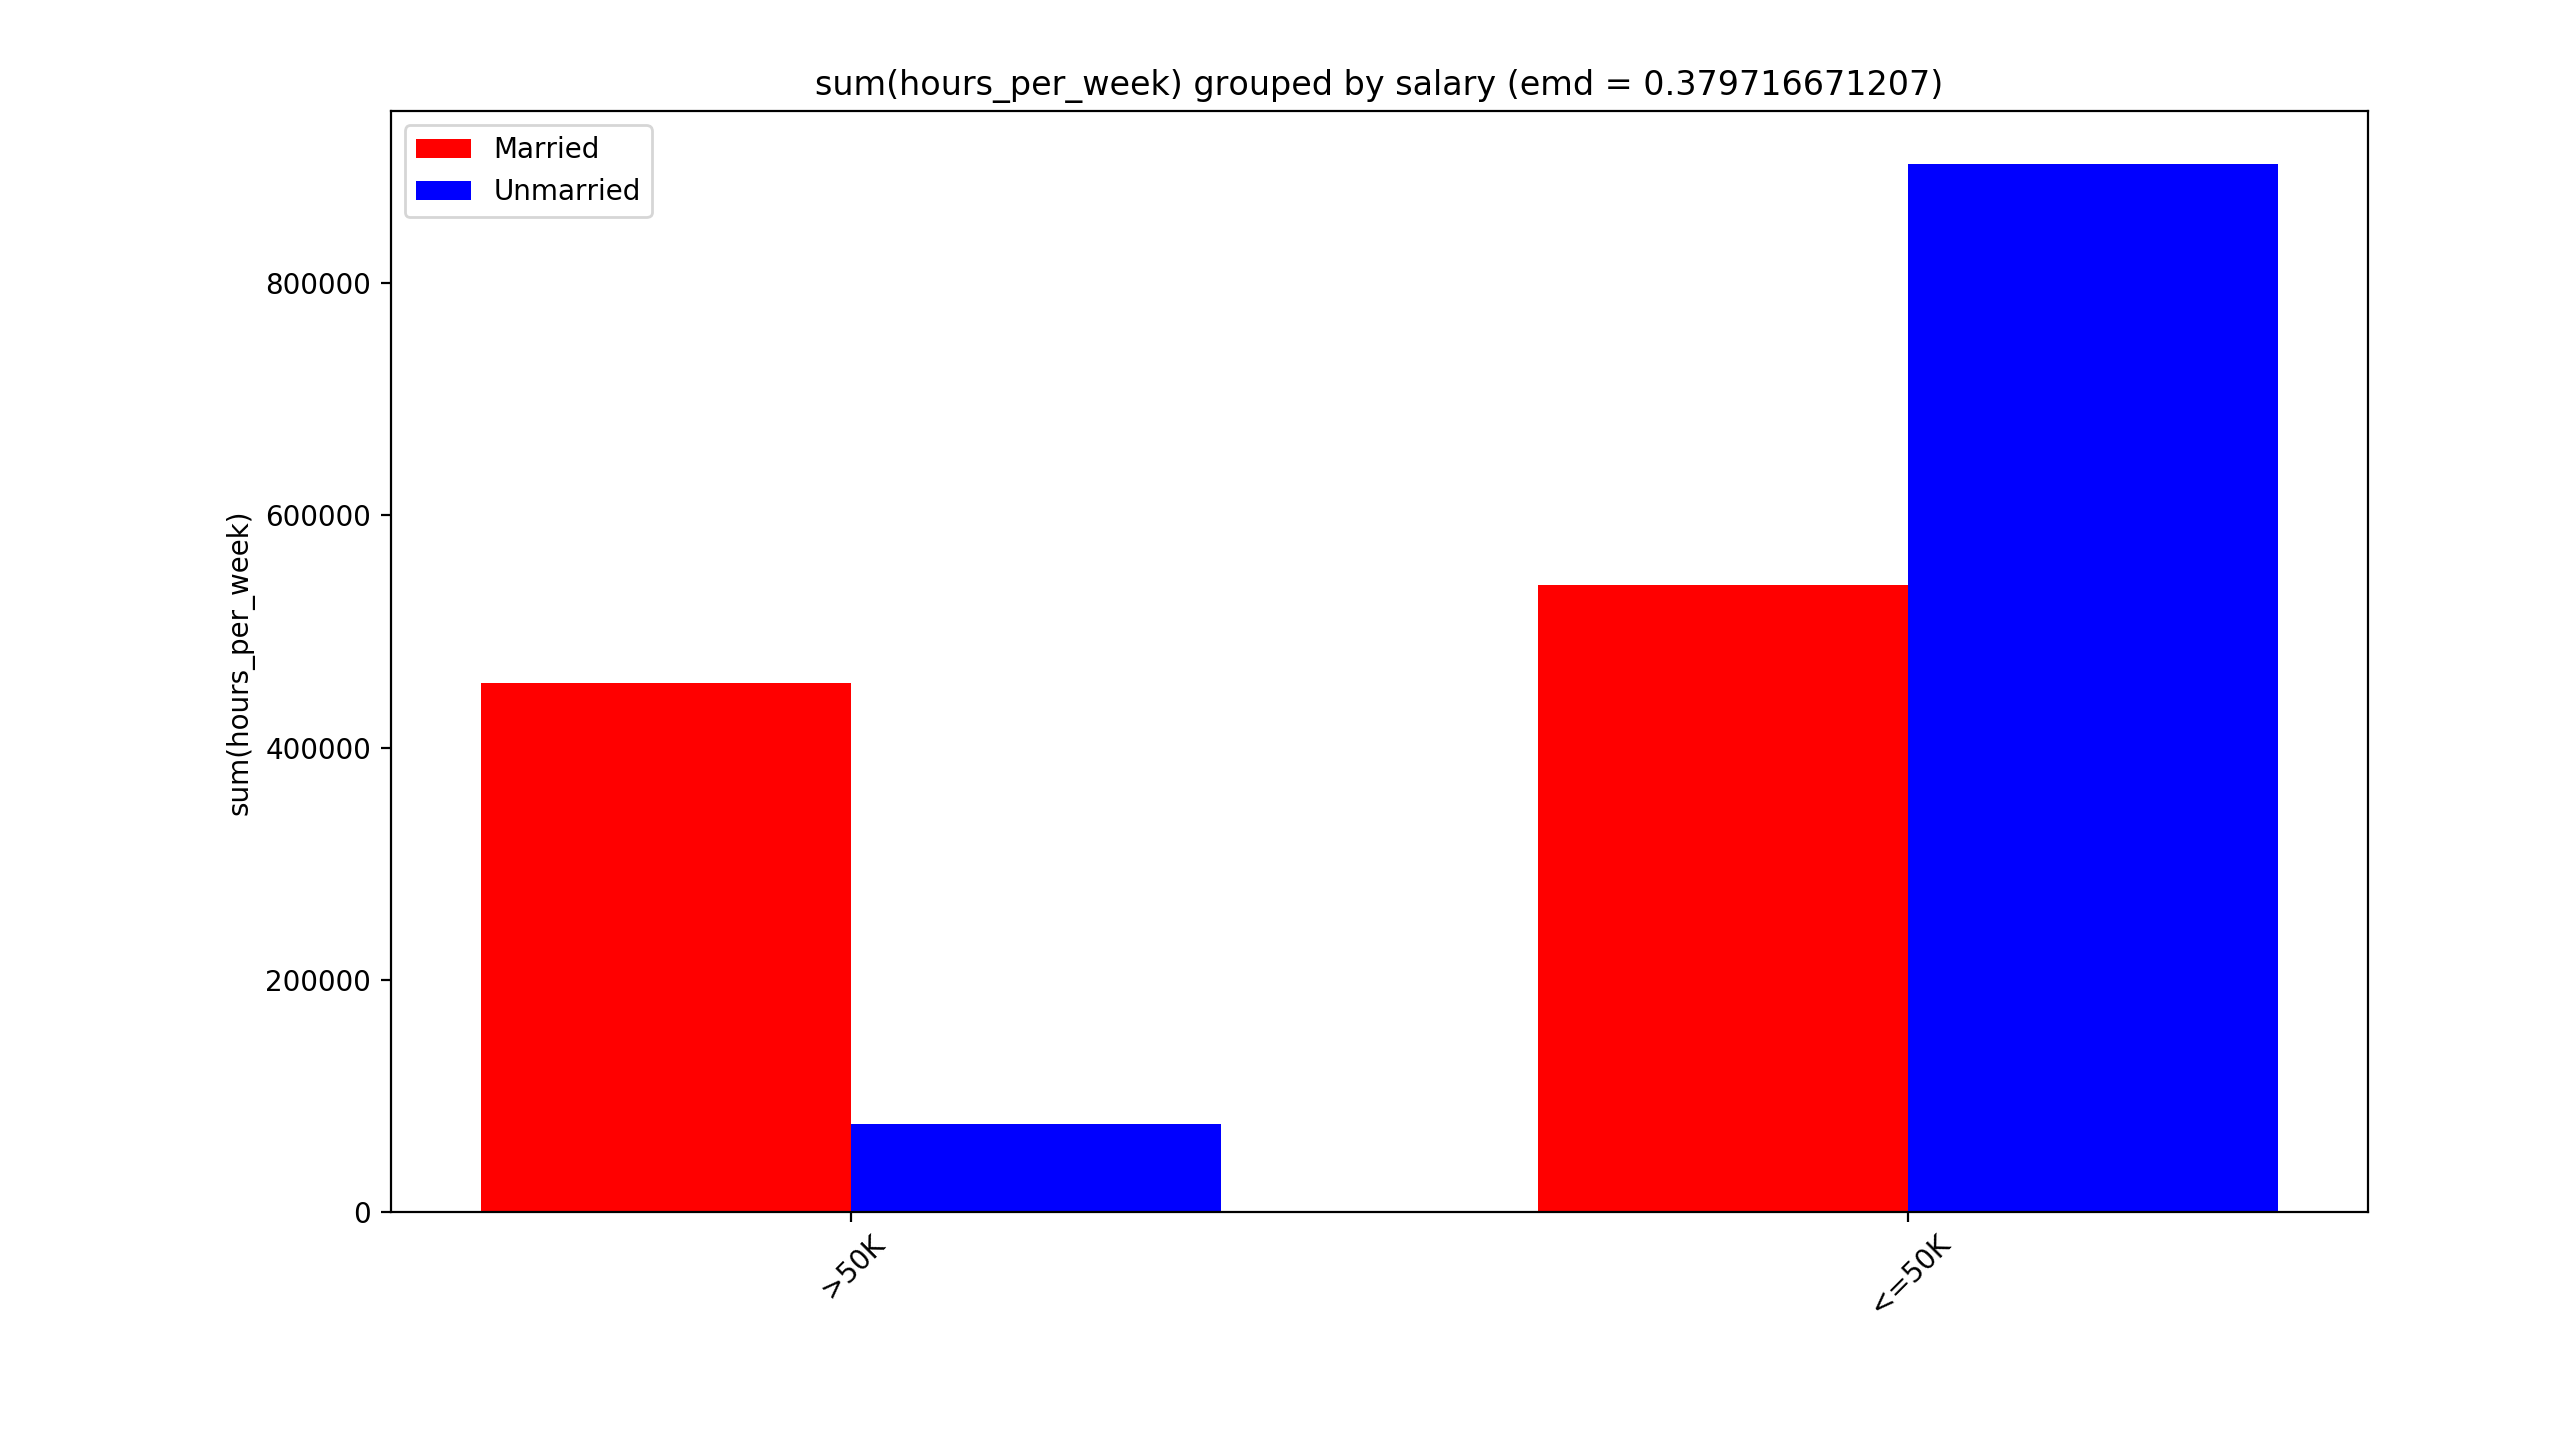
\includegraphics[scale=0.35]{figures/3salary_sum_fnlwgt_emd.png}
\end{figure}

\begin{figure}[h]
	\centering
	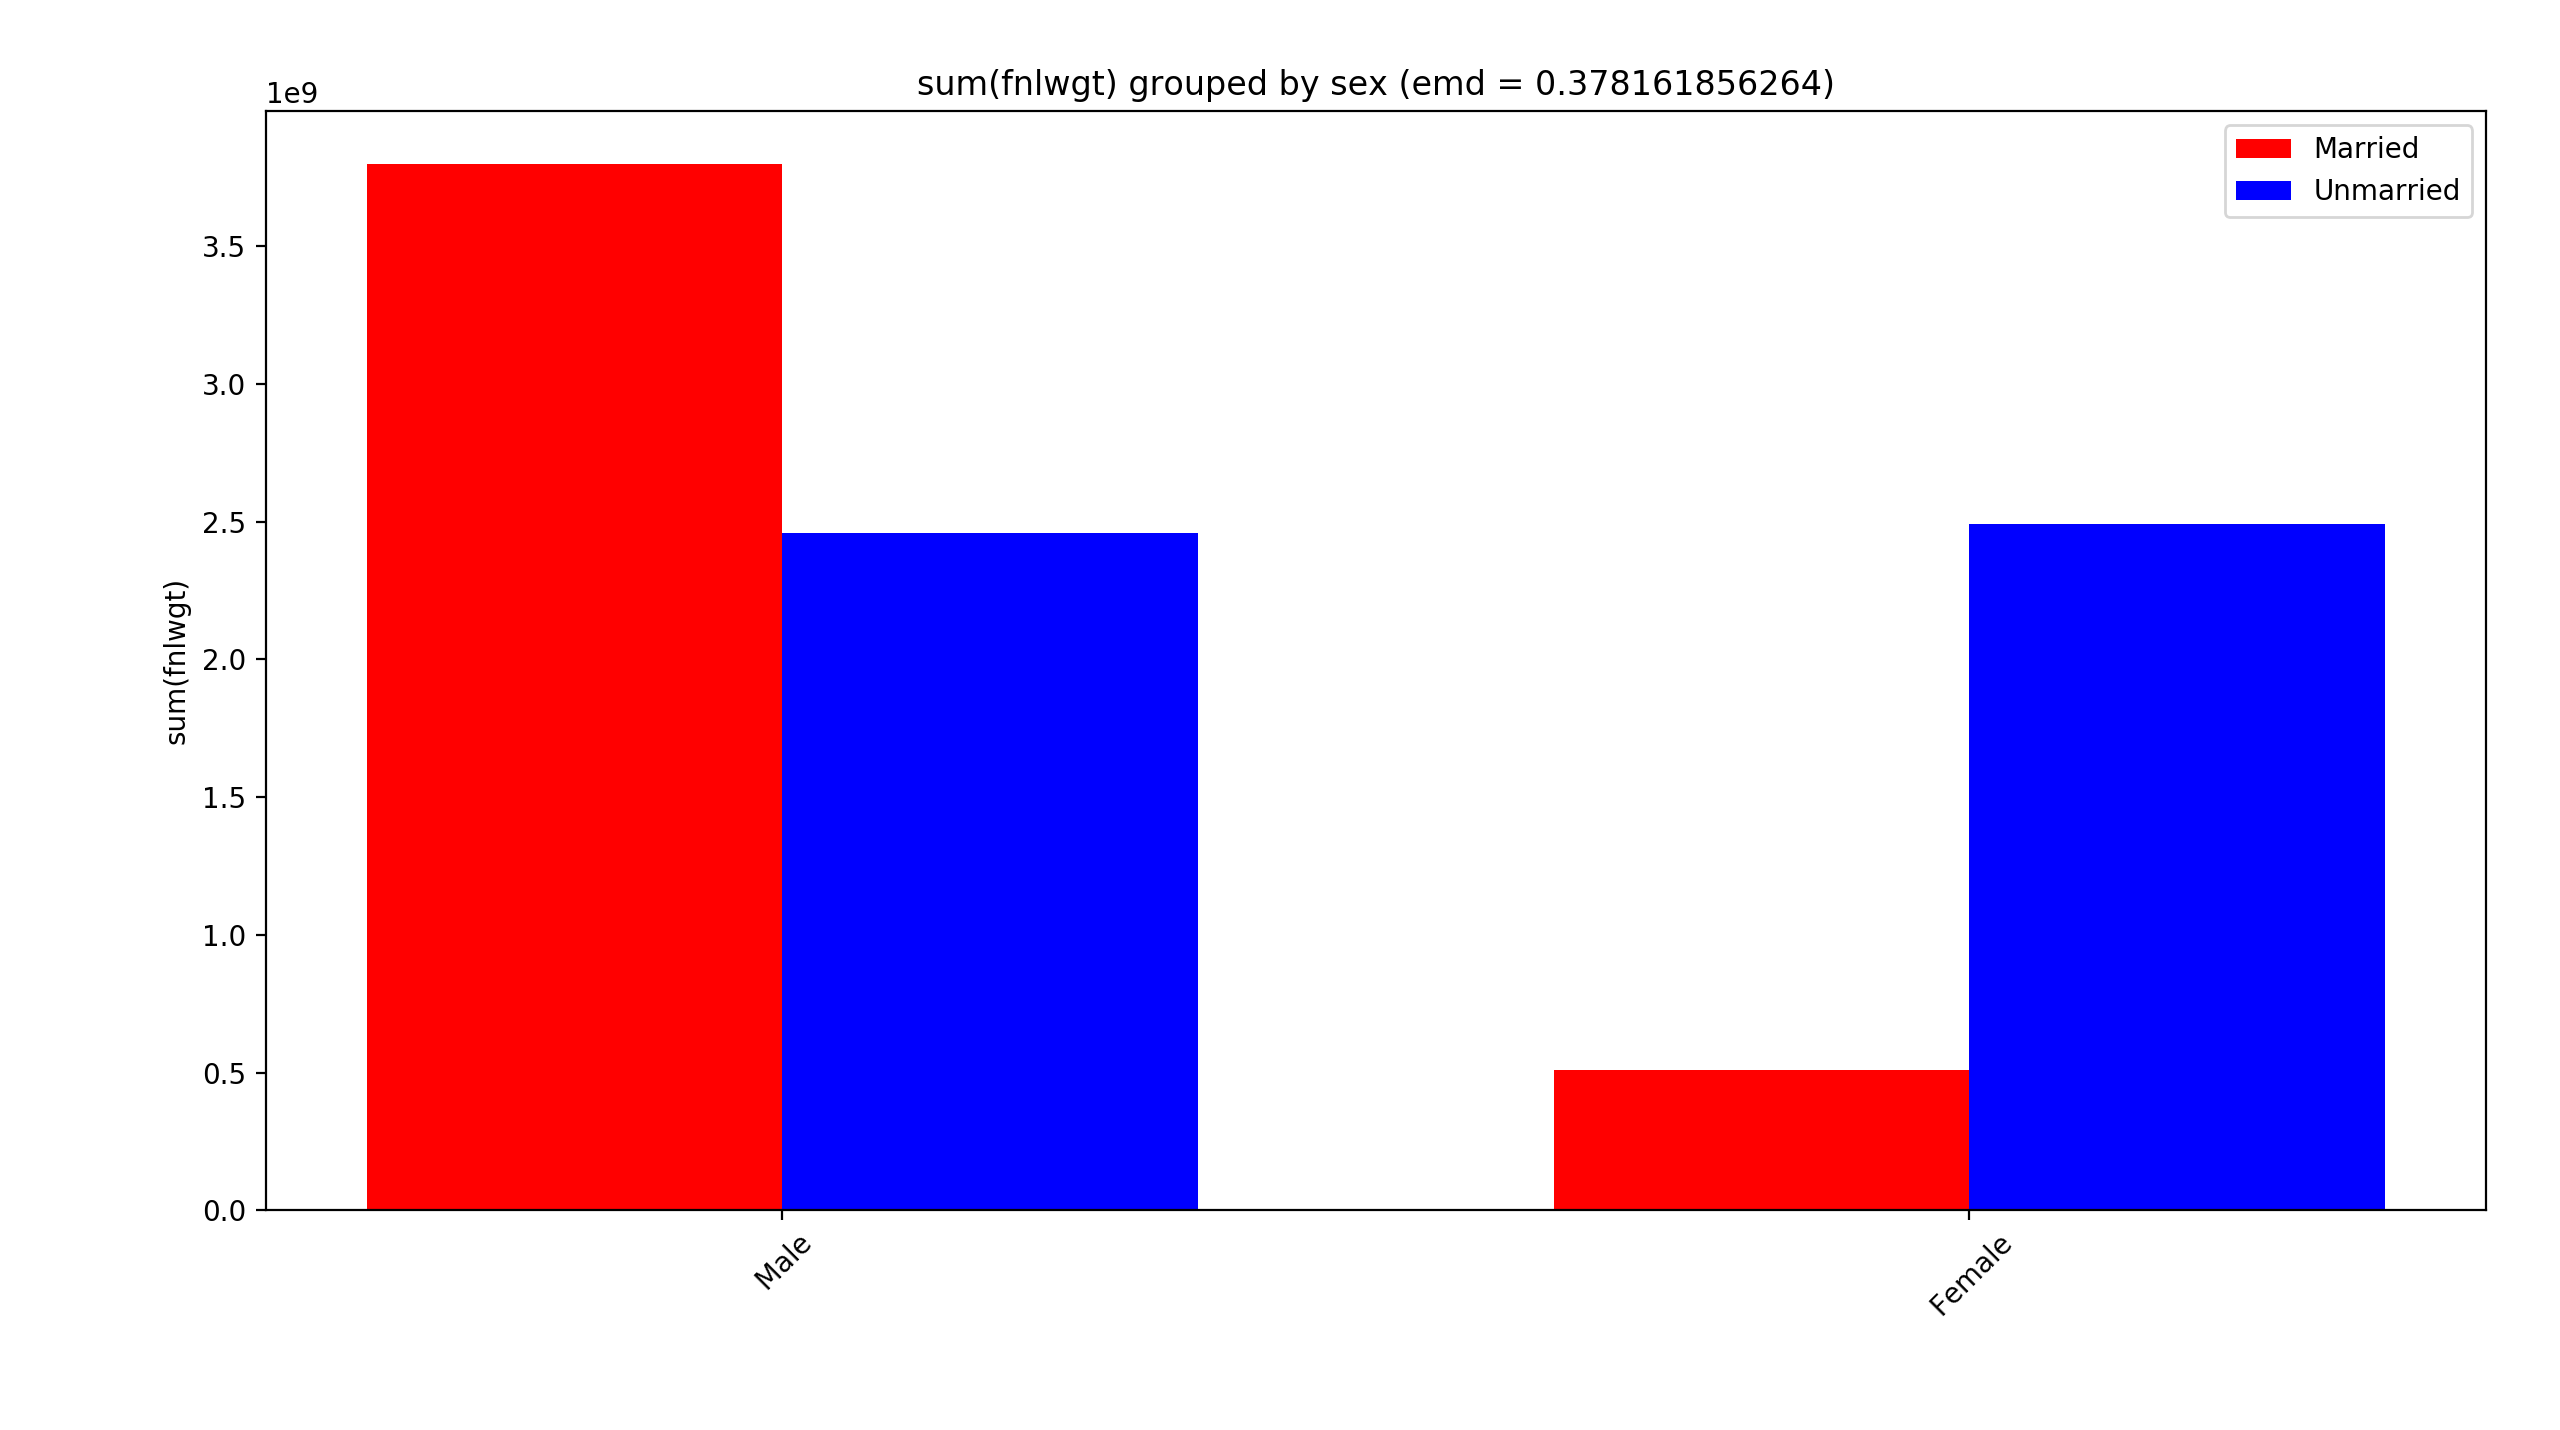
\includegraphics[scale=0.35]{figures/4sex_sum_fnlwgt_emd.png}
\end{figure}

\begin{figure}[h]
	\centering
	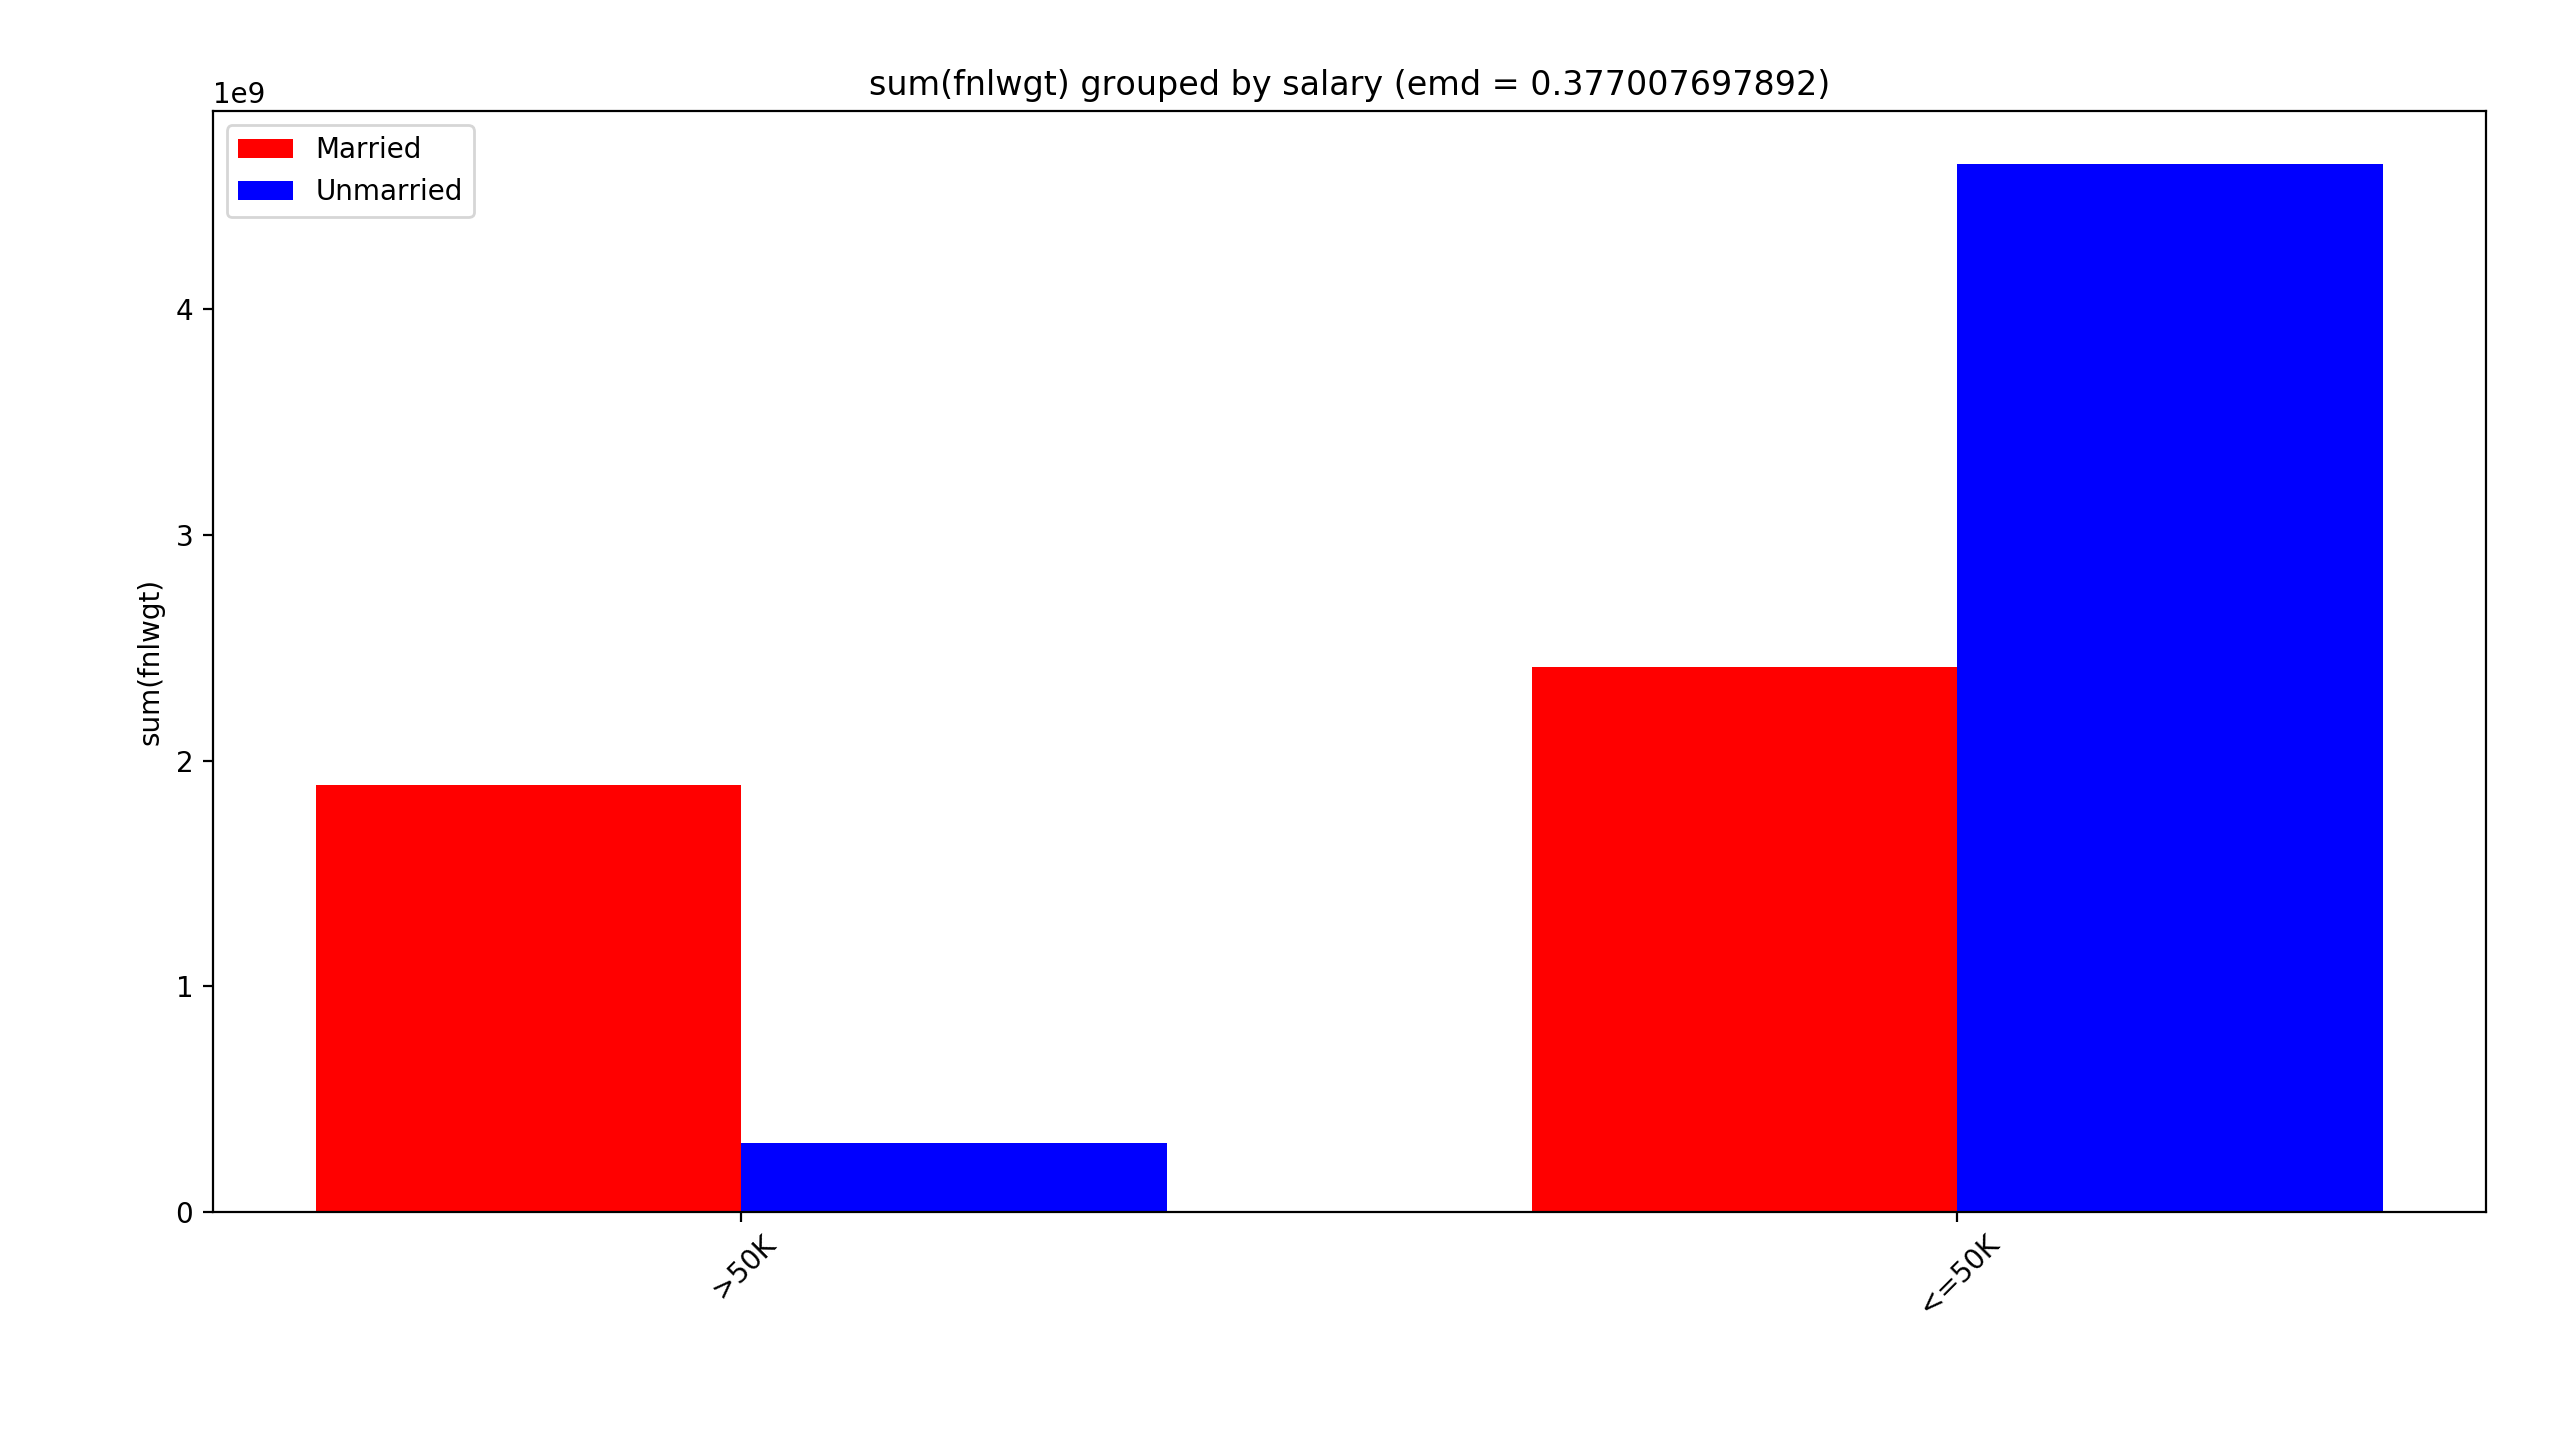
\includegraphics[scale=0.35]{figures/5salary_sum_fnlwgt_emd.png}
\end{figure}



\end{document}
